%!TEX root = ../thesis_phd.tex
%%%%%%%%%%%%%%%%%%%%%%%%%%%%%%%%%%%%%%%%%%%%%%%%%%%%%%%%%%%%%%%%%%%%%%%%%%%%%%%%
% event_selection.tex: Select of showering and tracking events:
%%%%%%%%%%%%%%%%%%%%%%%%%%%%%%%%%%%%%%%%%%%%%%%%%%%%%%%%%%%%%%%%%%%%%%%%%%%%%%%%
\chapter{Event Selection}
\label{event_selection_chapter}
%%%%%%%%%%%%%%%%%%%%%%%%%%%%%%%%%%%%%%%%%%%%%%%%%%%%%%%%%%%%%%%%%%%%%%%%%%%%%%%%

Measuring the parameters which govern a physical process requires
a clean sample of events which exhibit that process.
The definition of clean, of course varies wildly depending on the
experiment and parameters in question.
For this analysis, the goal is to accurately determine the reconstructed energy
spectrum for \numu CC events.
Thus, the goal of event selection is twofold: the selected sample should be
relatively background free and consist of events for which the energy of the
interacting neutrino can be determined.

Estimating the energy of events requires that they be fully contained
within the detector.
If all particles borne in the interaction deposit their energy within
the detector, then an estimate of the neutrino energy can be obtained using
the method described in section \ref{energy_section}.
If one or more of the particles escape the detector, it can be difficult
to estimate how much energy is missing.
Events with poor energy resolution can provide some sensitivity to oscillation
parameters, in particular \thetatth, which governs the amplitude of oscillation.
This analysis, however, makes no attempt at including escaping events.

Two primary backgrounds must be suppressed for this analysis.
The first is the vastly dominant cosmic-ray background; the FD is
on the surface of the earth rather than underground
and is thus exposed to cosmic rays at a rate in excess of 100 kHz \cite{tdr}.
The second is source of background is events from the \numi beam which are
not \numu CC interactions.
NC interactions are the trickiest beam background to reject due to their
abundance, especially those with a charged pion in the final state which
can produce a relatively long track.
Both appeared and survived \nue in the beam are relatively rare and tend
not to fake \numu CC signal.

The event classifier described in Chapter \ref{cnn_chapter} serves as to resolve
both cosmic-ray and beam-induced backgrounds.
Additional selection cuts described in this chapter serve to ensure
reconstruction quality and containment.
A handful of extra cuts are required to further reject cosmic background.


\begin{figure}
\begin{center}
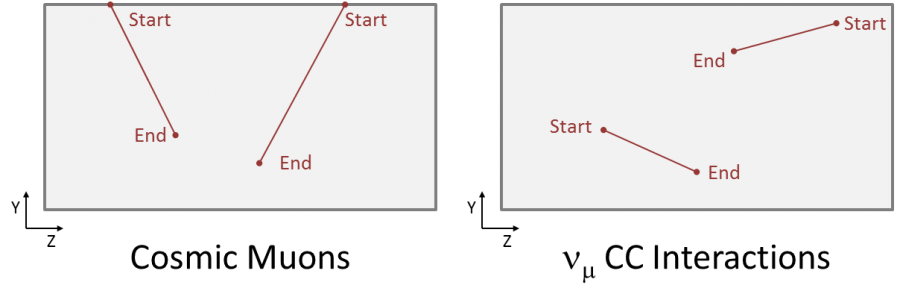
\includegraphics[width=0.95\textwidth]{figures/selection/cosmicmuons.png}
\end{center}
\caption{Comparison of track topologies for cosmic-ray and neutrino events}{
Cosmic-ray muon tracks (left) will tend to touch at least one detector face.
Neutrino interactions (right) which occur within the detector will tend to
be well contained.
Cosmic-ray tracks which touch two detector faces can be rejected without
appreciable signal loss.
}

\label{cosmictracks}
\end{figure}



\section{Cosmic-Ray Preselection}
\label{cosmicveto_section}

The vast abundance of cosmic-ray activity in the FD necessitates the
use of an initial preselection upstream of heavier reconstruction
algorithms.
Running the entire reconstruction chain over all cosmic-ray activity would
simply be too computationally expensive.
Instead, an initial preselection has been applied based on the output
of the slicing and CosmicTrack algorithms described in chapter
\ref{reconstruction_chapter}.
The preselection rejects roughly 90\% of cosmic-ray activity while preserving
nearly all contained \numu CC signal.

A large majority of cosmic-ray activity consists of muons which traverse the
detector, as depicted in Figure \ref{cosmictracks}.
If the muon tracks are well reconstructed, this activity can easily be rejected
by identifying tracks which touch two faces of the detector.
Proximity to the detector faces is determined by measuring the distance
between the track start and stop points as projected along the track
direction.
The track projections method is depicted in Figure \ref{trackproj}.
This measure is only reliable when the simple CosmicTrack fit has succeeded,
however.
The fit result is checked by assessing the fraction of hits in the slice
which were included in the track fit, with high values indicating a
successful fit.
As such, the event is rejected if both projected distances are less
than 35 cm and
the hit fraction is greater than 0.8.


\begin{figure}
\begin{center}
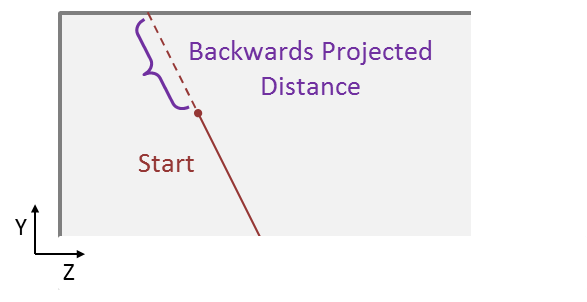
\includegraphics[width=0.7\textwidth]{figures/selection/backdist.png}
\end{center}
\caption{Illustration of track distance projection}{
The proximity of a track endpoint to the edge of the detector is determined
by measuring the distance projected along the track direction.
}
\label{trackproj}
\end{figure}

The cosmic-ray preselection also requires events to have at least 20 hits
and fewer than 400.  Events outside of that range are typically of an
interaction energy which carries little oscillation sensitivity.  An additional
selection variable is constructed from the track direction cosines relative to
the beam, $c_{beam}$, and vertical, $c_y$:
\begin{equation}
a = |c_{beam}| * (c_y + 1)
\end{equation}
Tracks from the CosmicTrack algorithm are constructed as downgoing, so $c_y$ is
always negative.  Thus, the variable $a$ is large, the track is generally
directed along the beam axis and not highly vertical.
Events with $a$ greater than 0.2 will pass the preselection.

\section{Reconstruction Quality}

Events of which have not been well reconstructed can cause problems
in energy estimation.
In particular, identification of the muon track within a \numu CC interaction
requires the KalmanTrack algorithm to have reconstructed a 3D track.
Events with very little activity are also not especially intelligible.
As such, the reconstruction quality selection requires a reconstructed track
from the CosmicTrack algorithm as well as a 3D track from the KalmanTrack
algorithm.
The quality selection also requires events to have at least 20 hits
spanning at least 4 contiguous planes.

\section{Muon Track Designation}

As described in Section \ref{energy_section}, reconstructed neutrino
energy depends on the identification of a muon track.
This distinction is made by the Muon ID algorithm described in Section
\ref{remid_section}.
Tracks reconstructed by the KalmanTrack algorithm
(Section \ref{kalmantrack_section}) are each assigned a Muon ID
score.
The track with the highest Muon ID score is dubbed the muon track
and treated with particular selection requirements.
All remaining activity in the slice is grouped into a hadronic
cluster, which also receives particular selection requirements.


\section{Containment}

\subsection{Far Detector Containment}

Containment in the FD is based on the distance of the slice and track
endpoints from the edges of the detector.
Slices are required to be at within the detector with a buffer of two
planes upstream and downstream as well as two cells in both views.
Track containment is based on projected distances in a similar fashion
to the cosmic-ray preselection, however the distances are measured in
the number of cells spanned by the projection rather than the distance itself.
The muon track is required to have a projected span of at least
11 cells in the forward and backward direction, and at least one cell
for the track from CosmicTrack.

\subsection{Near Detector Containment}

Containment in the ND is more complicated than the FD due to the consideration
of the Muon Catcher and its truncated height.
Slices are rejected if they start in the first two planes of the detector or
end within the last two planes.
The muon track is required to start in active region by requiring that
the start $Z$ position is within 1175 cm from the front of the detector.
If a track enters the muon catcher, the height of the track
at the first muon catcher plane is required to be less than the height of
the muon catcher ($Z = 55$ cm) to ensure that it did not leave and re-enter
the detector.
The track projection is also required to span at least five cells in the
forward direction nine cells in the backward direction.
Finally, the hadronic cluster (all hits in the slice not on the muon track)
is required to have calorimetric energy less than 30 MeV.


\section{Background Rejection}
\label{background_rejection_section}

The selections above ensure events are of sufficient quality for analysis
and reduce level of cosmic-ray activity to an acceptable level.
The primary rejection of NC and cosmic-ray events is handled by
the convolutional neural network classifier and some additional requirements
to handle cosmic-ray events which would remain in the sample otherwise.

The convolutional neural network discriminant is formed by the sum of the four
softmax outputs corresponding to \numu CC (QE, RES, DIS, other).
Events are rejected if the softmax output is less than 0.5.
Figure \ref{cvnnumu} shows the distribution of the discriminant for
signal and background.
A fair amount of cosmic-ray background slips past the softmax requirement.
The vast majority of these events are near the top of the detector
and can be rejected by requiring the CosmicTrack start $Y$ position to be less
than 600 cm, as seen in Figure \ref{cosStartY}.
Additional cosmic background can be rejected using the transverse momentum
of the event.
Two measures of transverse momentum are used, one which is based
on the reconstructed slices and another based on the reconstructed prongs
described in \cite{niner2015thesis}.
In the slice method, a unit vector is formed in the direction running
from the start of the muon track to the energy centroid of the slice;
the transverse momentum fraction reconstructed as the sine of the angle
between that vector and the beam axis.
The prong method is similar, except that the the momentum vector
is formed as the energy weighted sum of all reconstructed prongs
for that slice.
Both of these transverse momentum measures, seen in Figures \ref{tranMom} and
\ref{pngptp}, are required to be less than 0.8.



\begin{figure}
\begin{center}
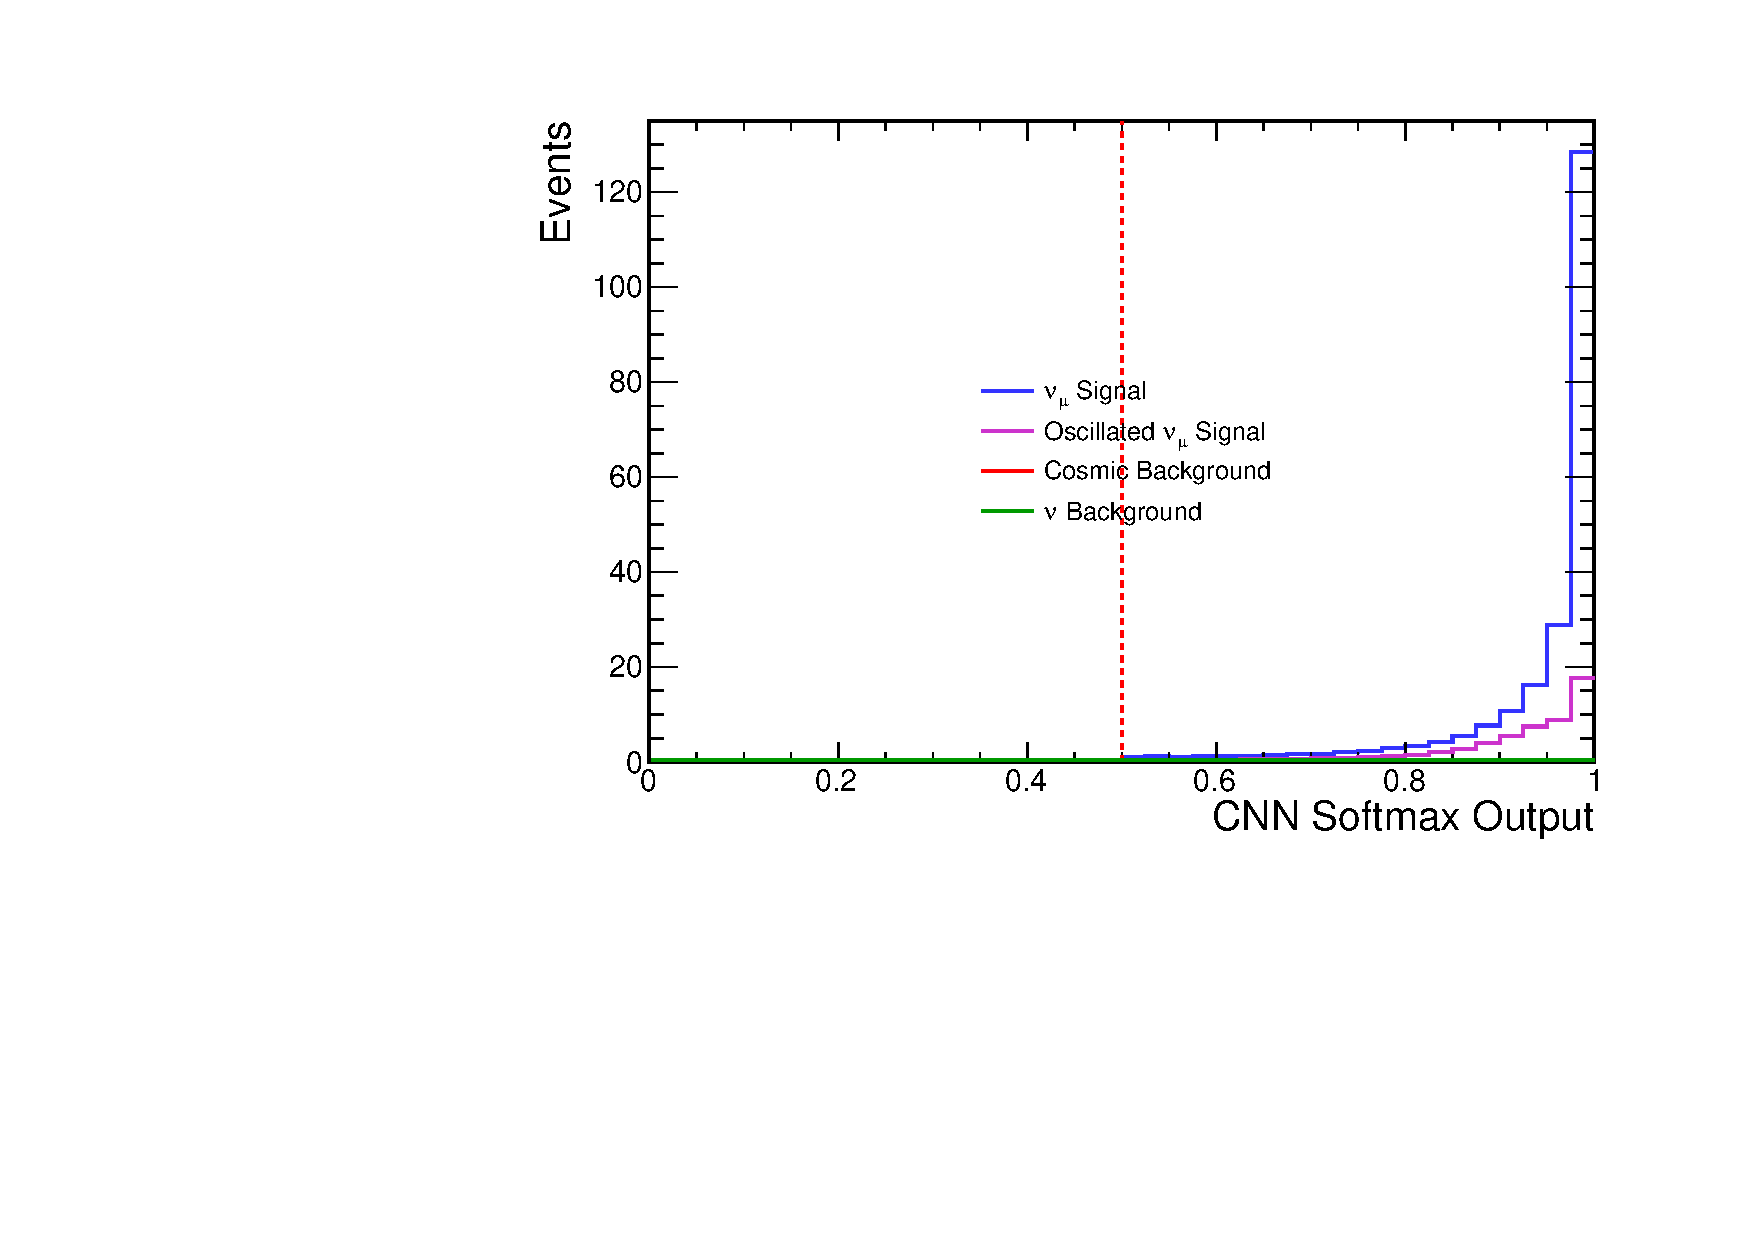
\includegraphics[width=0.9\textwidth]{figures/selection/n1_cvnnumu.pdf}
\end{center}
\caption{Distribution of softmax output from convolutional neural network for signal and backgrounds}{
The convolutional neural network output serves as the primary discriminant for
rejecting background.
The blue distribution shows \numu CC signal from the unoscillated beam spectrum,
magenta shows the oscillated spectrum (weighted according to Section
\ref{osc_weight_section}).
The red and green distributions show the cosmic-ray and beam backgrounds,
respectively.
Selection applied to these distributions include all FD analysis cuts
with the exception of the cut on the variable shown here.
Events are rejected if they fall to the left of the vertical
dashed red line.
}
\label{cvnnumu}
\end{figure}


\begin{figure}
\begin{center}
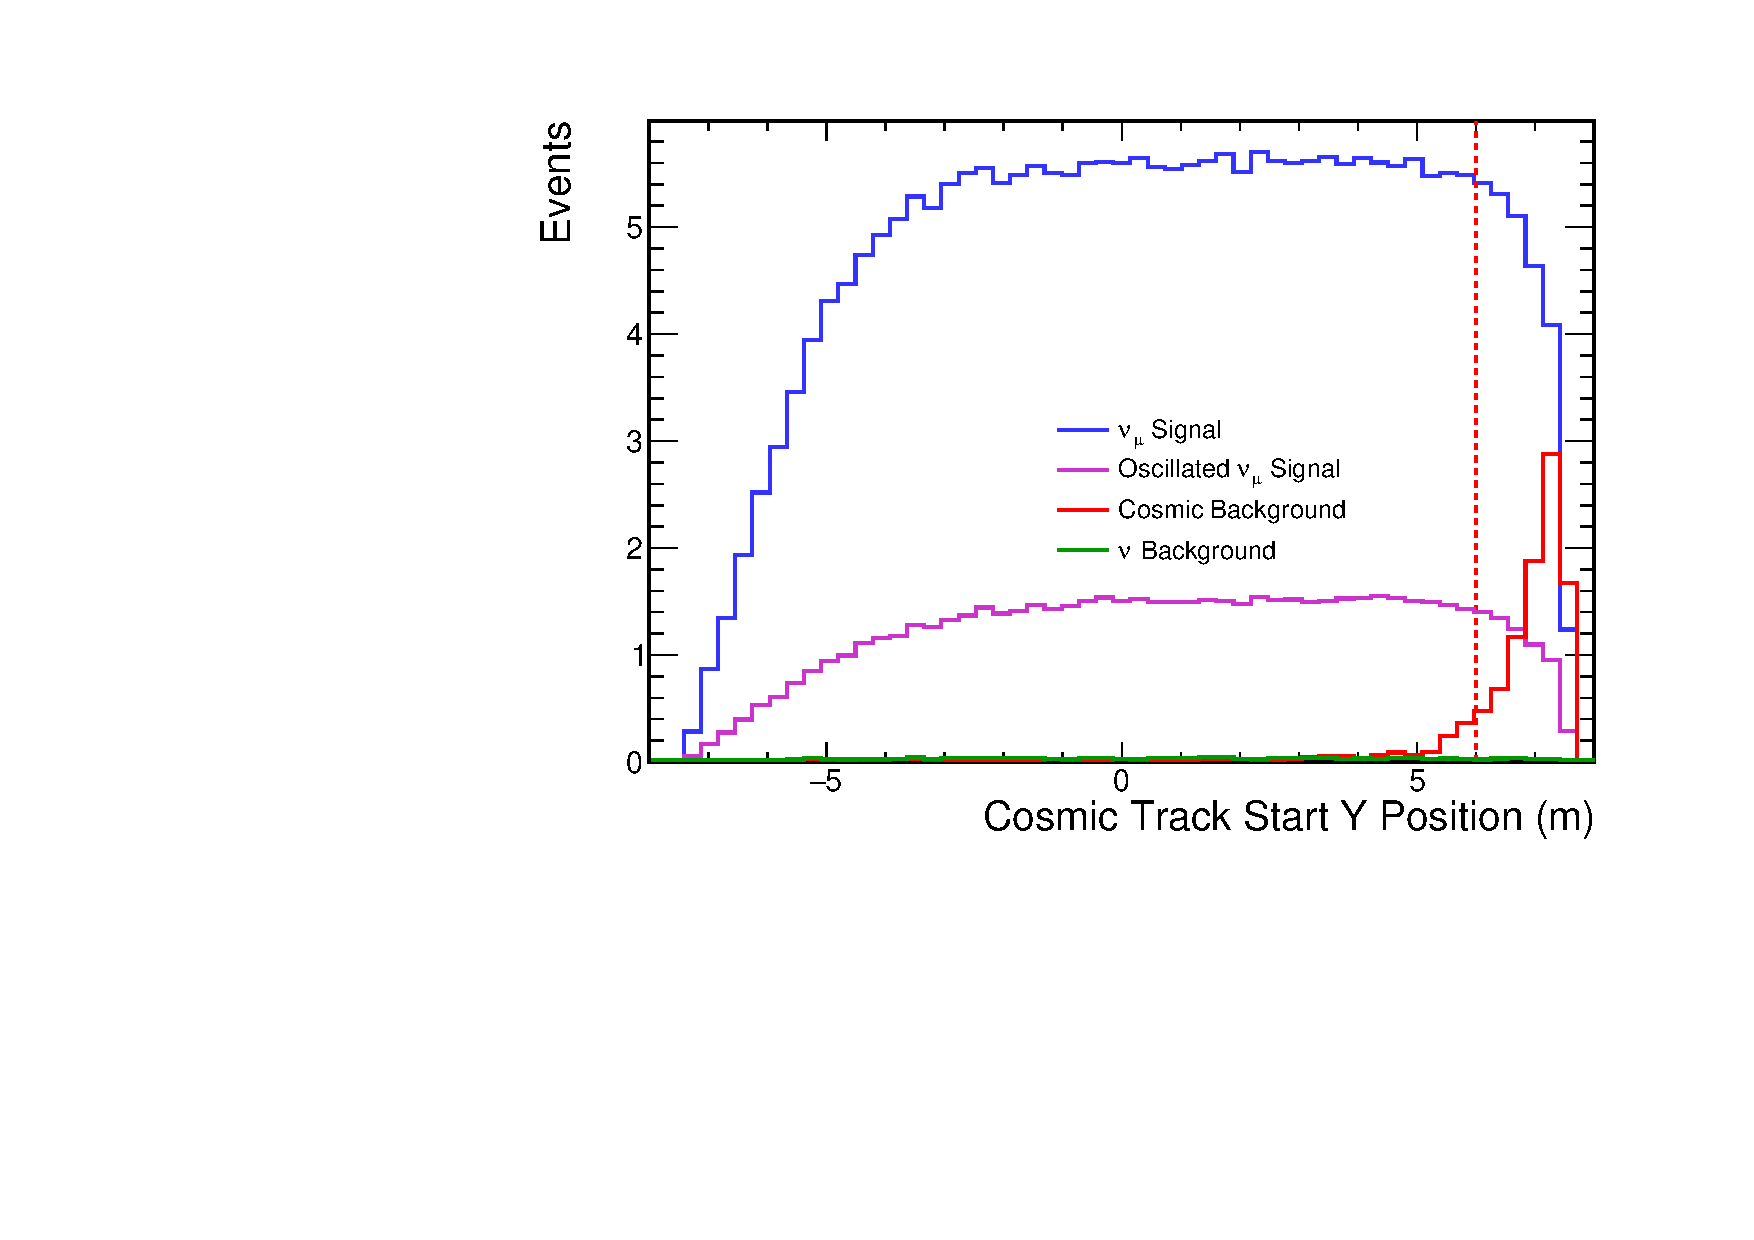
\includegraphics[width=0.9\textwidth]{figures/selection/n1_cosStartY.pdf}
\end{center}
\caption{Distribution of CosmicTrack start $Y$ position for signal and backgrounds}{
The blue distribution shows \numu CC signal from the unoscillated beam spectrum,
magenta shows the oscillated spectrum (weighted according to Section
\ref{osc_weight_section}).
The red and green distributions show the cosmic-ray and beam backgrounds,
respectively.
Selection applied to these distributions include all FD analysis cuts
with the exception of the cut on the variable shown here.
Events are rejected if they fall to the right of the vertical
dashed red line.
}
\label{cosStartY}
\end{figure}

\begin{figure}
\begin{center}
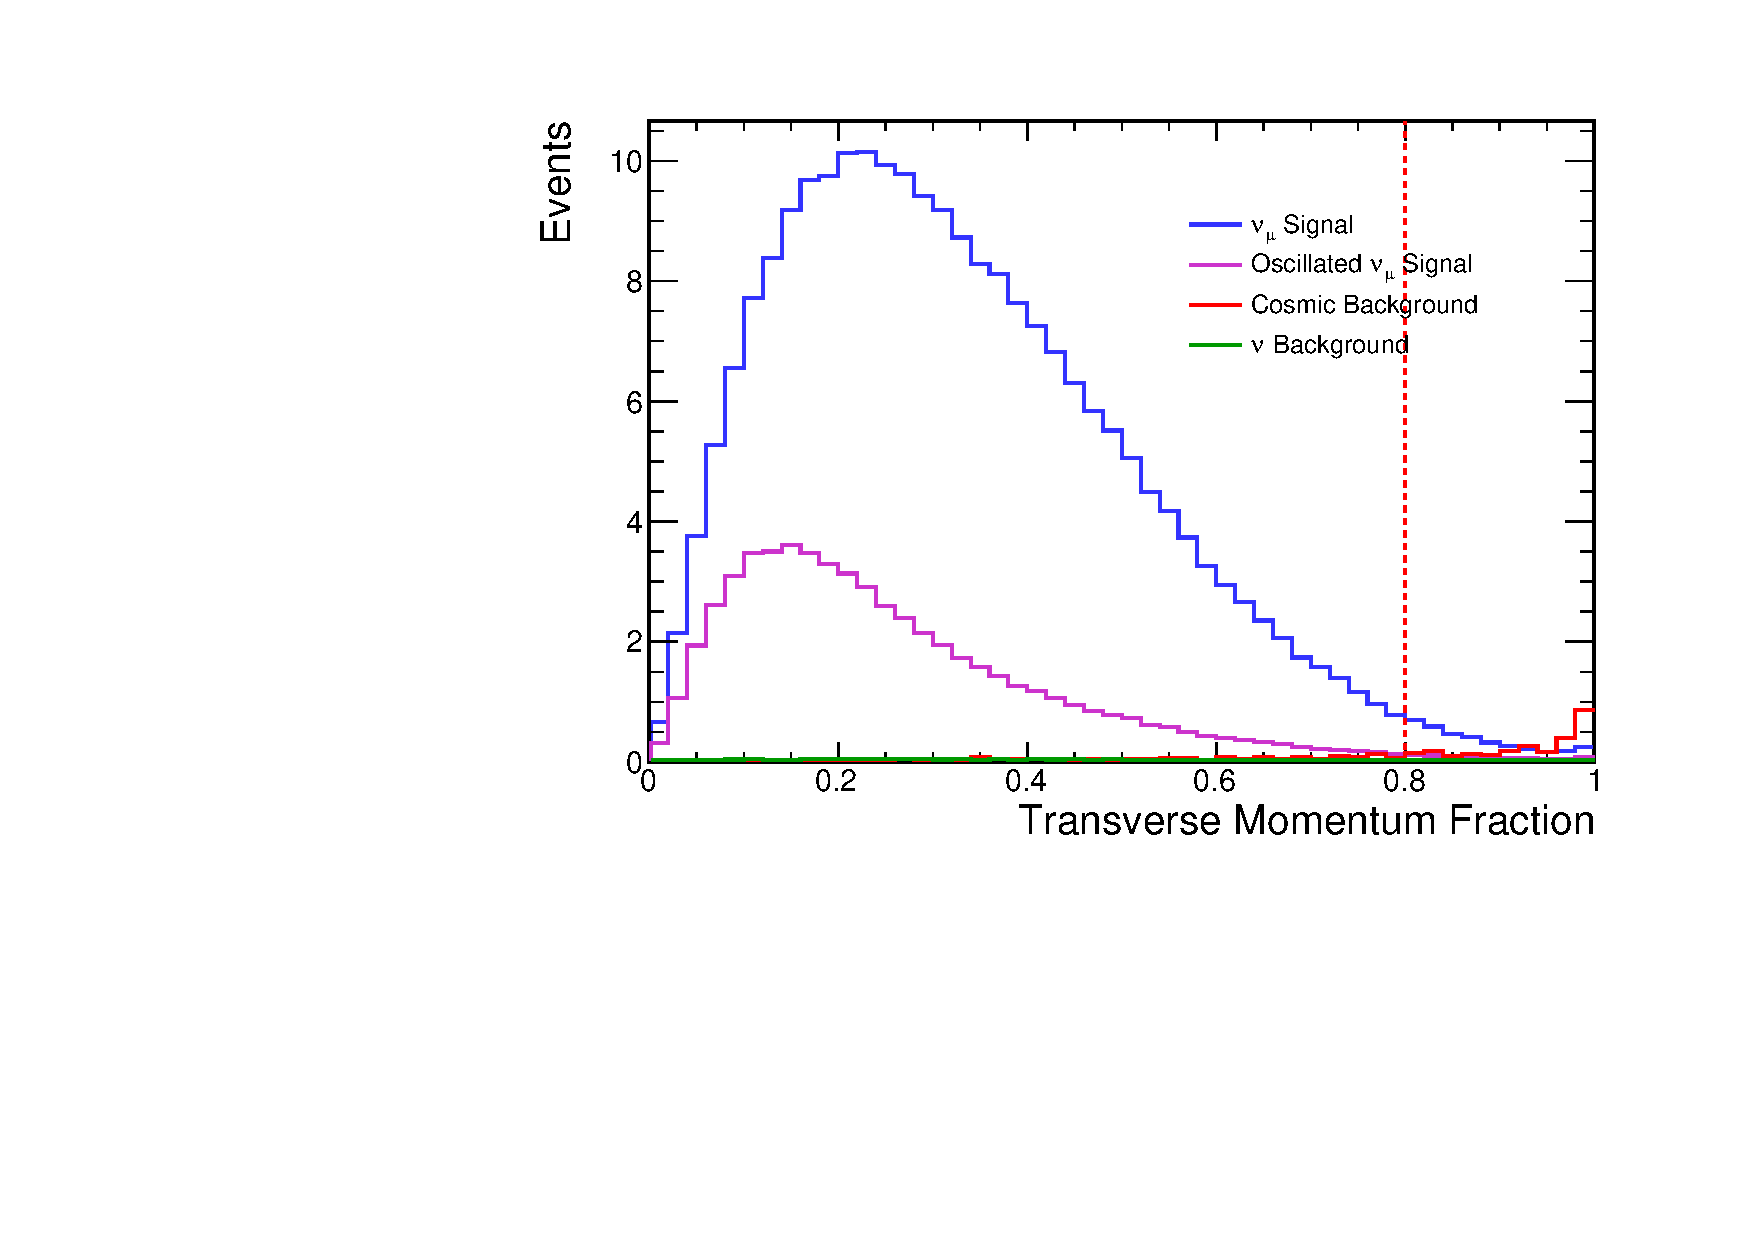
\includegraphics[width=0.9\textwidth]{figures/selection/n1_tranMom.pdf}
\end{center}
\caption{Distribution of transverse momentum estimated from slice mean position
for signal and backgrounds}{
The blue distribution shows \numu CC signal from the unoscillated beam spectrum,
magenta shows the oscillated spectrum (weighted according to Section
\ref{osc_weight_section}).
The red and green distributions show the cosmic-ray and beam backgrounds,
respectively.
Selection applied to these distributions include all FD analysis cuts
with the exception of the cut on the variable shown here.
Events are rejected if they fall to the right of the vertical
dashed red line.
}
\label{pngptp}
\end{figure}

\begin{figure}
\begin{center}
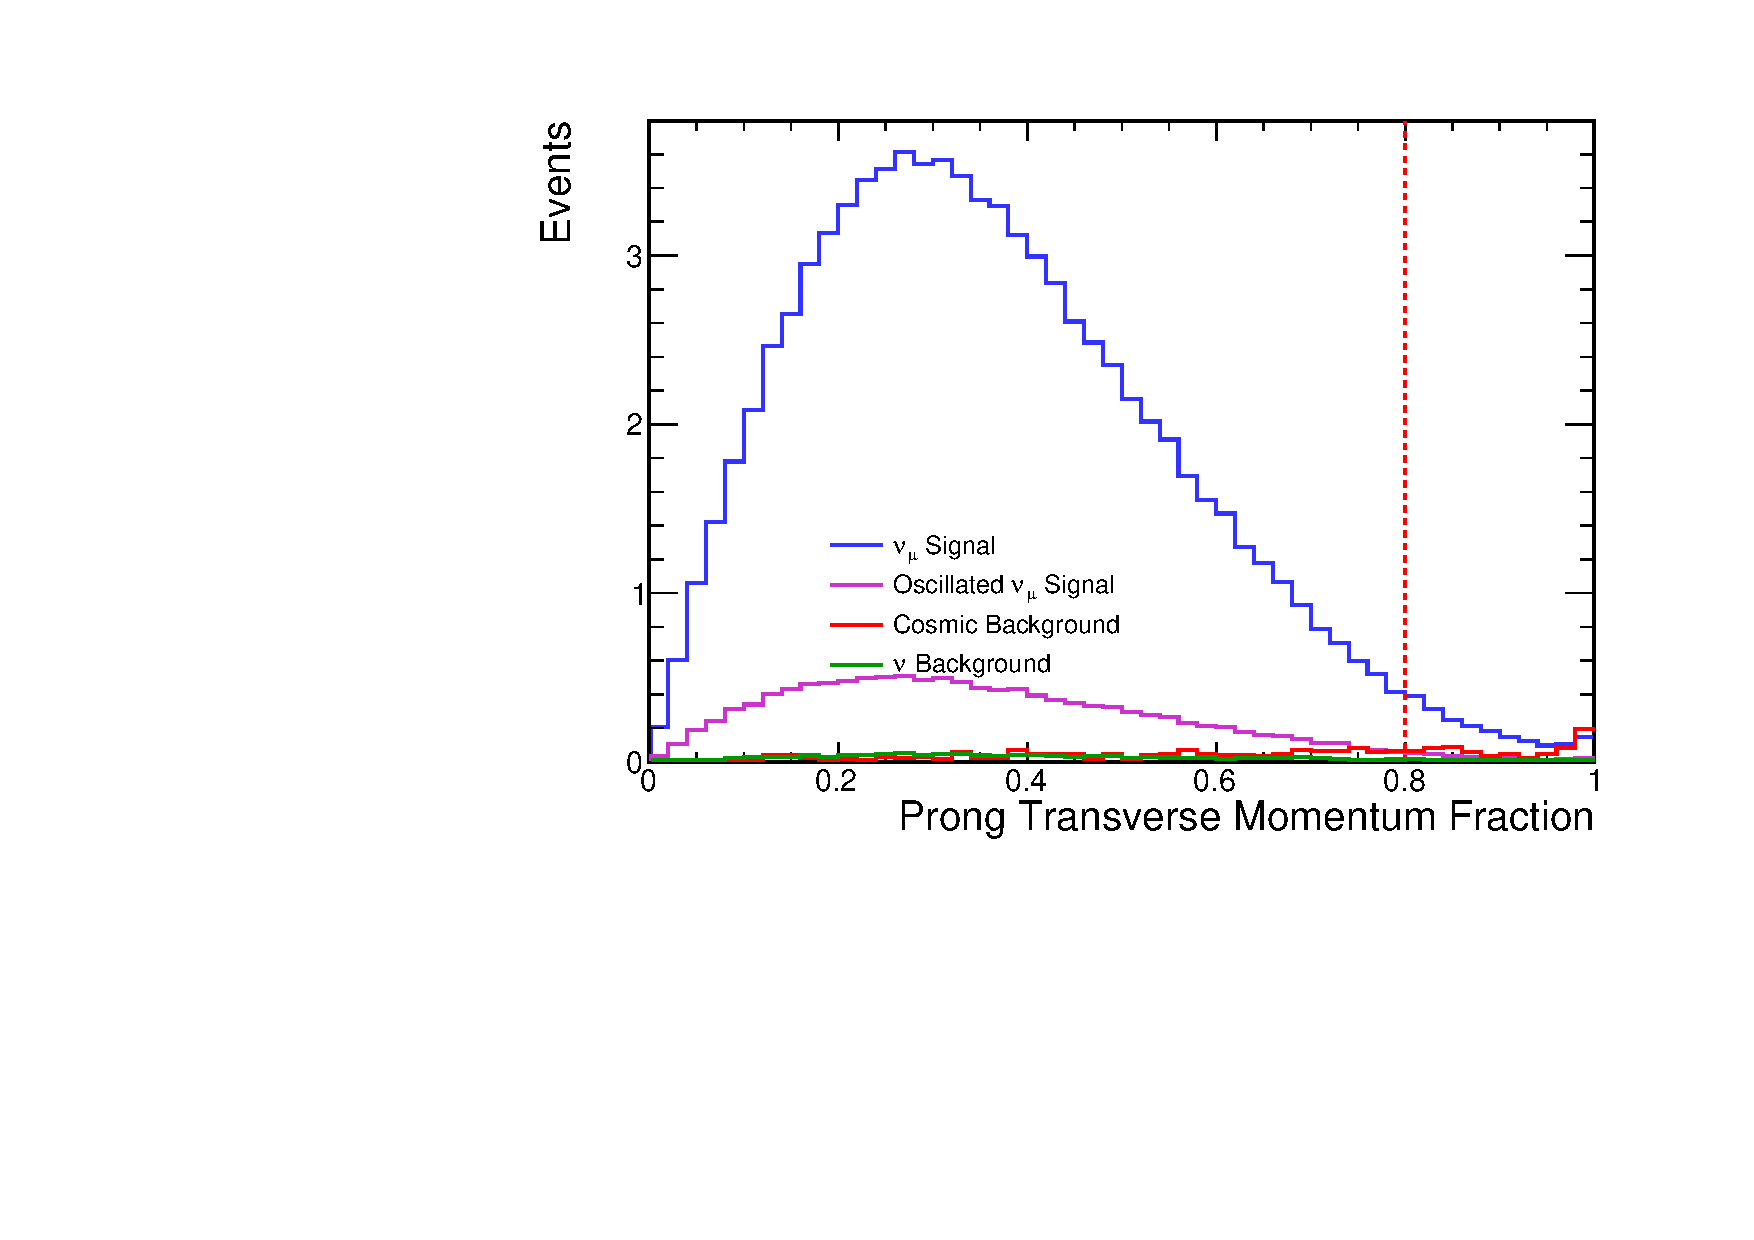
\includegraphics[width=0.9\textwidth]{figures/selection/n1_pngptp.pdf}
\end{center}
\caption{Distribution of transverse momentum estimated from reconstructed prongs
 for signal and backgrounds}{
The blue distribution shows \numu CC signal from the unoscillated beam spectrum,
magenta shows the oscillated spectrum (weighted according to Section
\ref{osc_weight_section}).
The red and green distributions show the cosmic-ray and beam backgrounds,
respectively.
Selection applied to these distributions include all FD analysis cuts
with the exception of the cut on the variable shown here.
Events are rejected if they fall to the right of the vertical
dashed red line.
}
\label{tranMom}
\end{figure}


\section{FD Selected Sample}
\label{fd_selection_section}

The figures at the end of this chapter give many representations on the
FD selected sample.
Figure \ref{final_selection} shows FD MC prediction for
the reconstructed energy spectrum for the final selected energy spectrum.
Beyond that, two perspectives can be used to interpret the selection:
the selected spectrum itself and the efficiency of the selection.
In each bin, efficiency is the ratio of the selected events
to the total events which could have been selected.
The distribution denominator in this ratio -- events which could have been
selected -- is taken to be the sample of events with are contained
in the detector based on MC truth.
Simulated events are deemed to be contained if all true simulated energy
depositions are contained within the detector volume.
Figures \ref{cut_flow_sig}, \ref{cut_flow_bkg}, \ref{cut_flow_comp_sig}, and
\ref{cut_flow_comp_bkg} all include both MC prediction for the selected
FD spectrum and the efficiency ratio.
In the spectrum, the true contained events is shown as a black distribution,
which serves as the denominator for the efficiency distribution.

Figure \ref{cut_flow_sig} shows distriutions for true signal
events for the samples
remaining after each cut (quality, containment, CNN classifier,
CosmicTrack start
$Y$, and the two transverse momentum cuts) are successively applied.
Figure \ref{cut_flow_bkg} shows the same plots for the true background events.
For the CNN classifier, the signal efficiency is generally higher (~70\%)
for events with higher energy.
The CosmicTrack Start $Y$ cut leads to a flat reduction in signal efficiency
as a function of energy, which is to be expected since it simply reduces
the effective detector volume.
Transverse momentum, on the other hand, impacts low-energy events more
significantly since small reconstruction is more difficult for events
with less activity.
Cutting on the CNN classifier output reduces the background rate significantly,
as seen in figure \ref{cut_flow_bkg}.

Figures \ref{cut_flow_comp_sig} and \ref{cut_flow_comp_bkg} show
schematically similar plots, but the final two samples
are the result of different selections rather than applied separately.
The \textit{CNN + Cuts} sample uses the selection described here,
while \textit{Muon ID + BDT} uses the selection described in
\cite{nova2016numu}.
That alternative selection uses the presence of an identified muon
to select \numu CC events, as well as a boosted decision tree (BDT)
\cite{friedman2002stochastic} to reject cosmic-ray background.
The CNN approach provides improved efficiency in the low energy bins
which are especially sensitive to neutrino oscillation.
Losses in the high energy region are driven mainly by the CosmicTrack
start $Y$ cut.
Senitivity enhancement achieved by the CNN approach is quantified
in Figure \ref{contour_improvement}.


\begin{figure}
\begin{center}
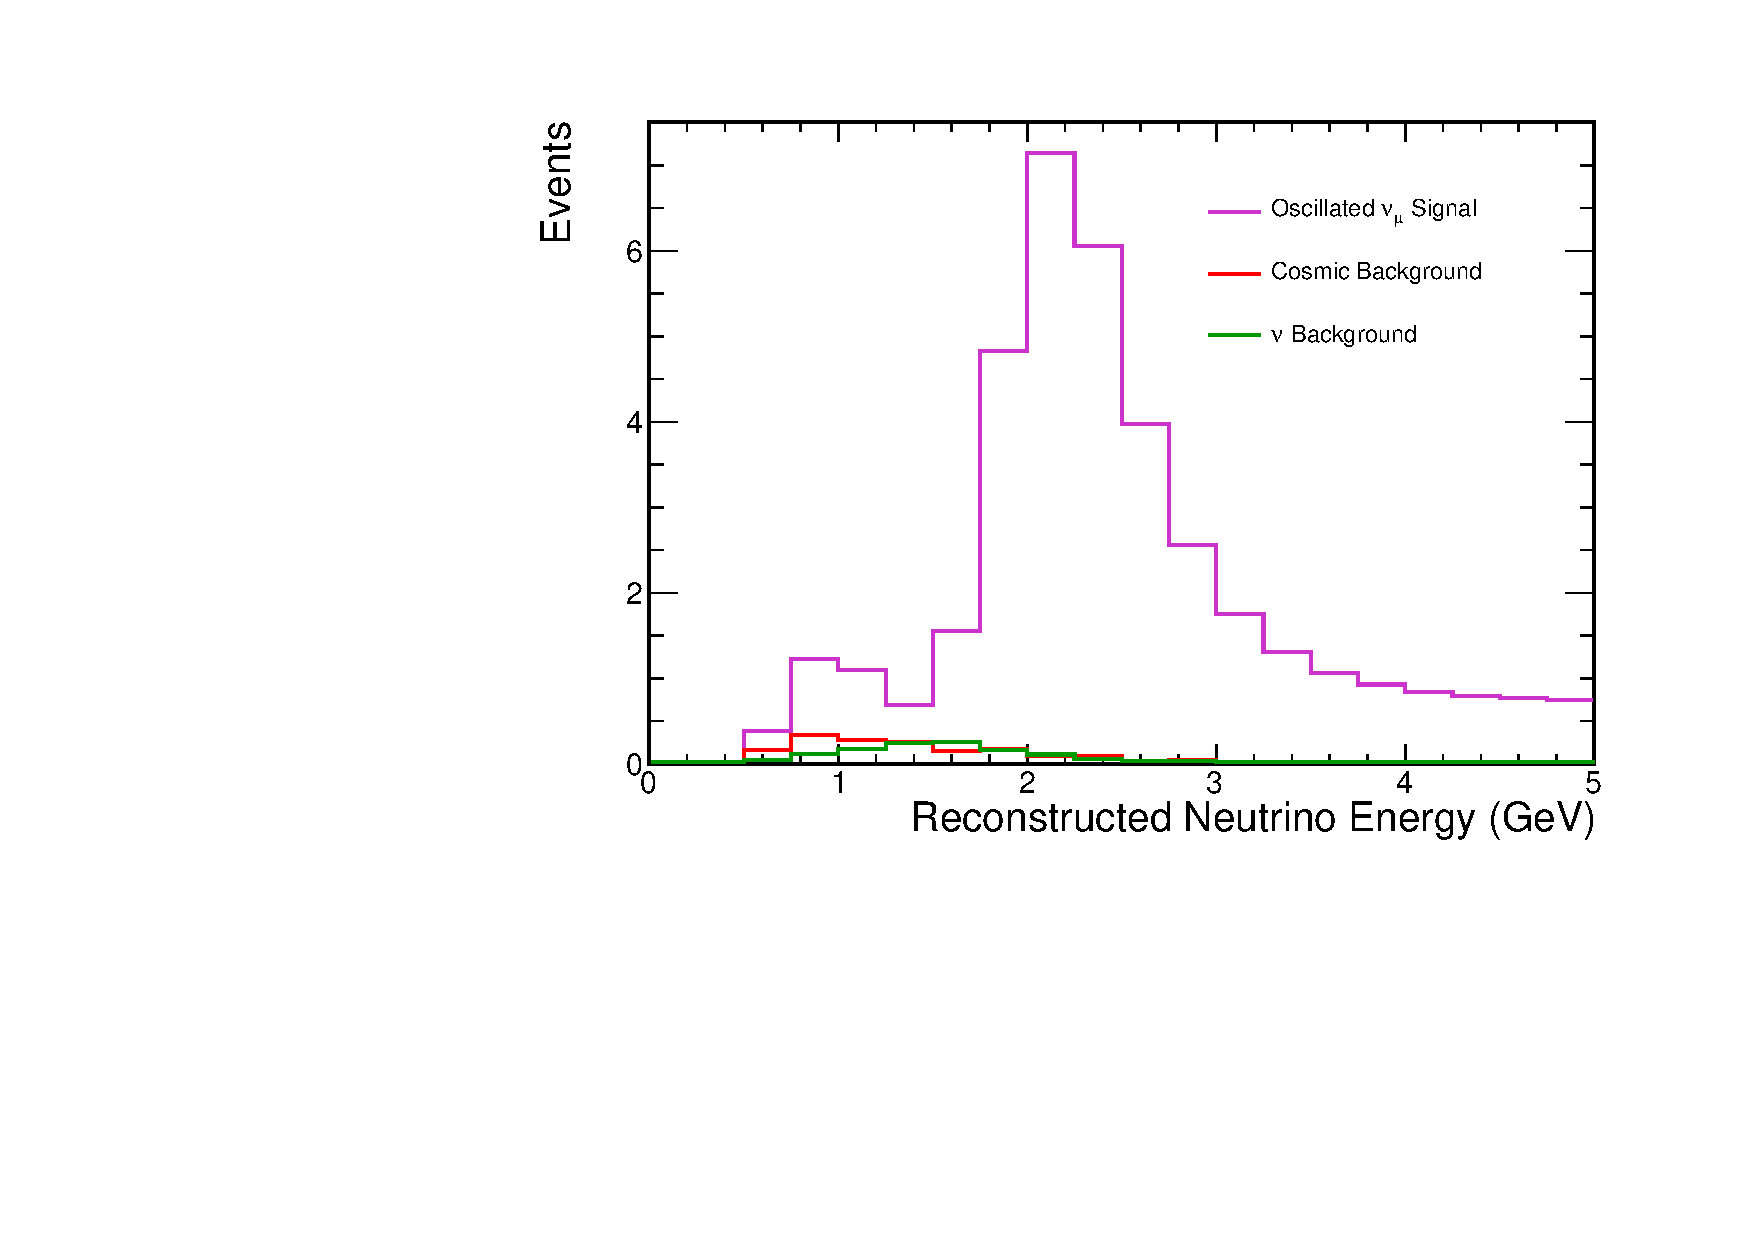
\includegraphics[width=0.9\textwidth]{figures/selection/numuE.pdf}
\end{center}
\caption{Final selected spectrum for \numu CC signal and backgrounds }{
The FD MC prediction of the final selected spectrum resulting from all cuts
described in this chapter.
The \numu CC signal distribution has had oscillation probabilities applied
based on the true energy of selected events and oscillation parameters
from described in \ref{osc_weight_section}.
}
\label{final_selection}
\end{figure}



\begin{figure}
\vspace{-30pt}
\begin{center}
  \begin{subfigure}[b]{0.7\textwidth}
    \centering
    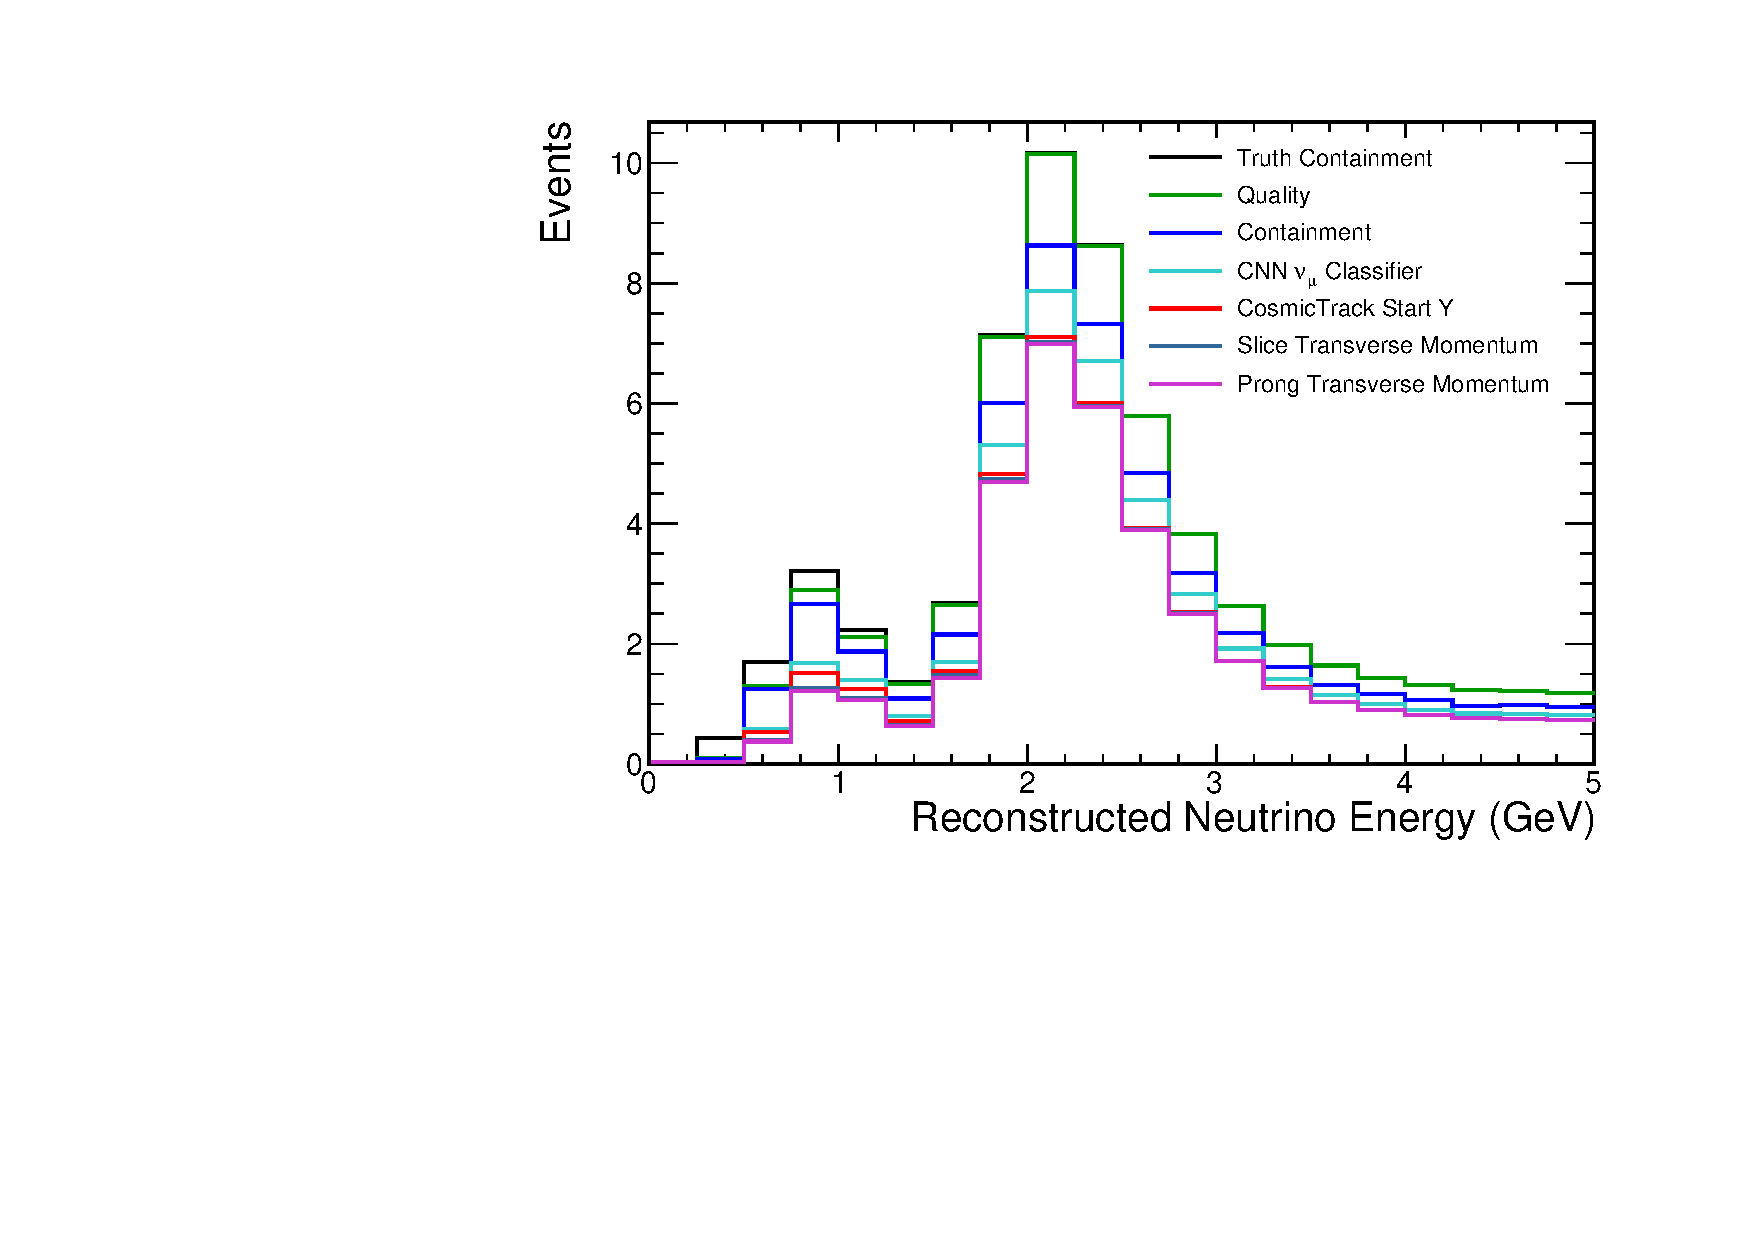
\includegraphics[width=\textwidth]{figures/selection/myflow_sig_osc.pdf}
  \end{subfigure}

  \begin{subfigure}[b]{0.7\textwidth}
    \centering
    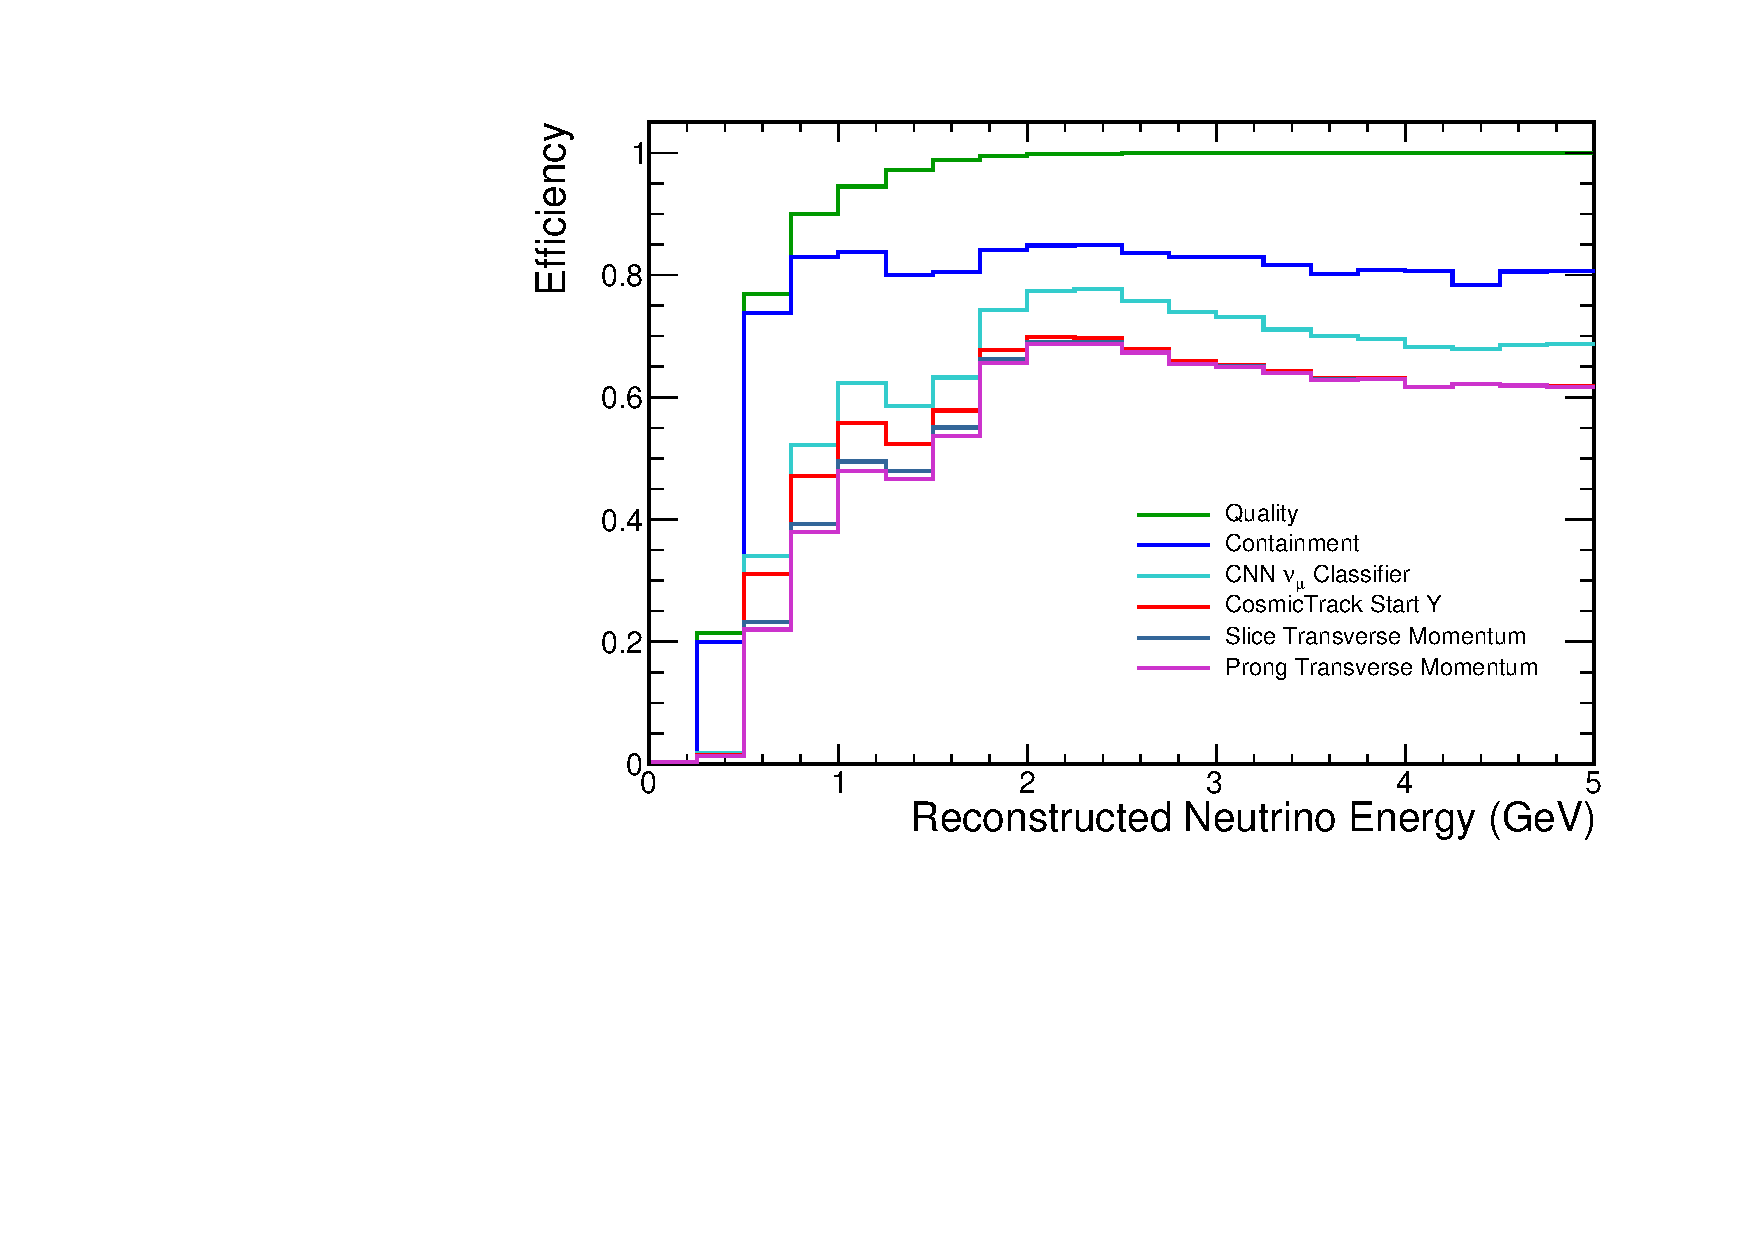
\includegraphics[width=\textwidth]{figures/selection/myflow_sig_eff_osc.pdf}
  \end{subfigure}

\end{center}
\vspace{-10pt}
\caption{Selected \numu CC signal event spectrum and efficiency}{
The top pane shows the reconstructed neutrino energy spectrum
for selected \numu CC signal events from FD MC simulation.
Truth containment is the sample of events which deposit
no energy outside of the detector, this serves as the denominator
for the efficiency ratio shown in the bottom pane.
Each subsequent spectrum adds an additional selection cut to the sample.
The \numu CC signal distribution has had oscillation probabilities applied
based on the true energy of selected events and oscillation parameters
from described by \ref{osc_weight_section}.
}
\label{cut_flow_sig}
\end{figure}


\begin{figure}
\vspace{-30pt}
\begin{center}
  \begin{subfigure}[b]{0.7\textwidth}
    \centering
    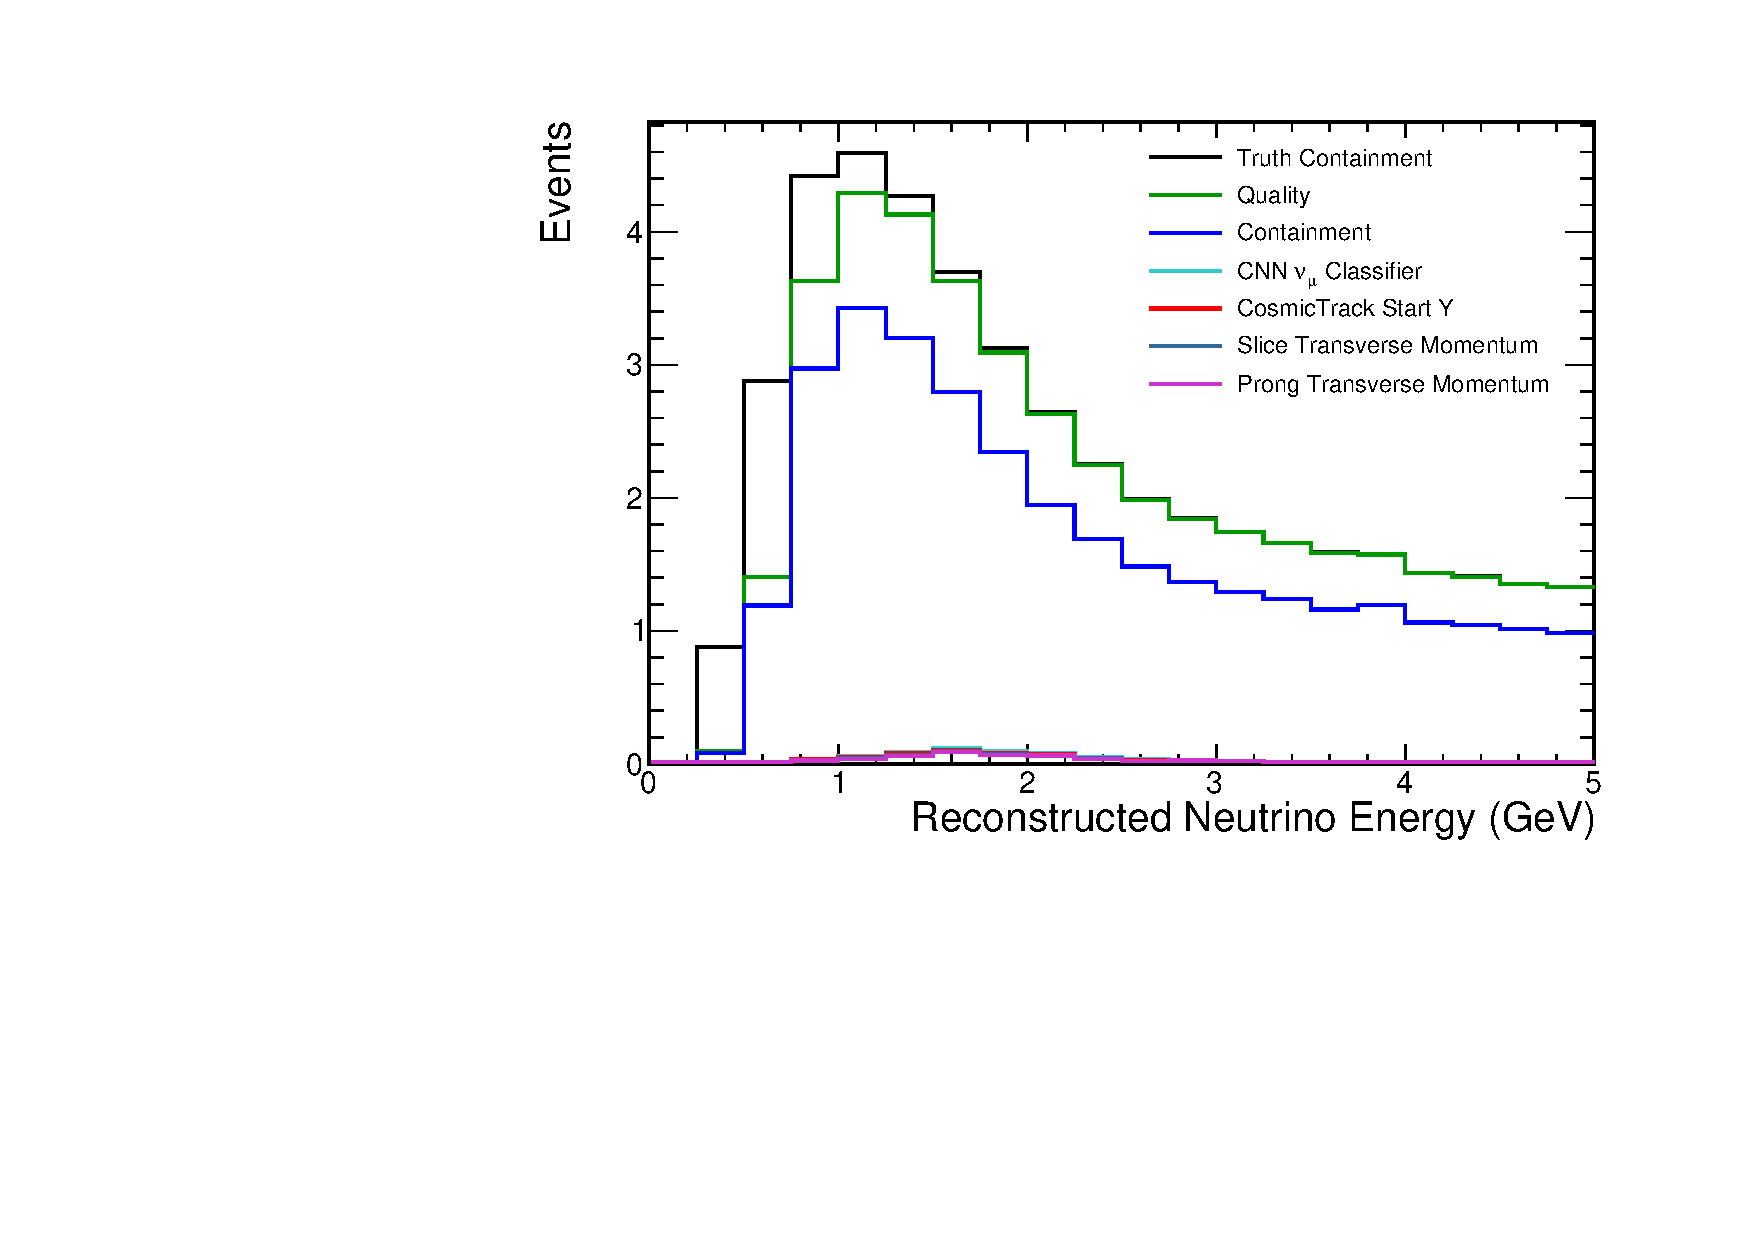
\includegraphics[width=\textwidth]{figures/selection/myflow_bkg_osc.pdf}
  \end{subfigure}

  \begin{subfigure}[b]{0.7\textwidth}
    \centering
    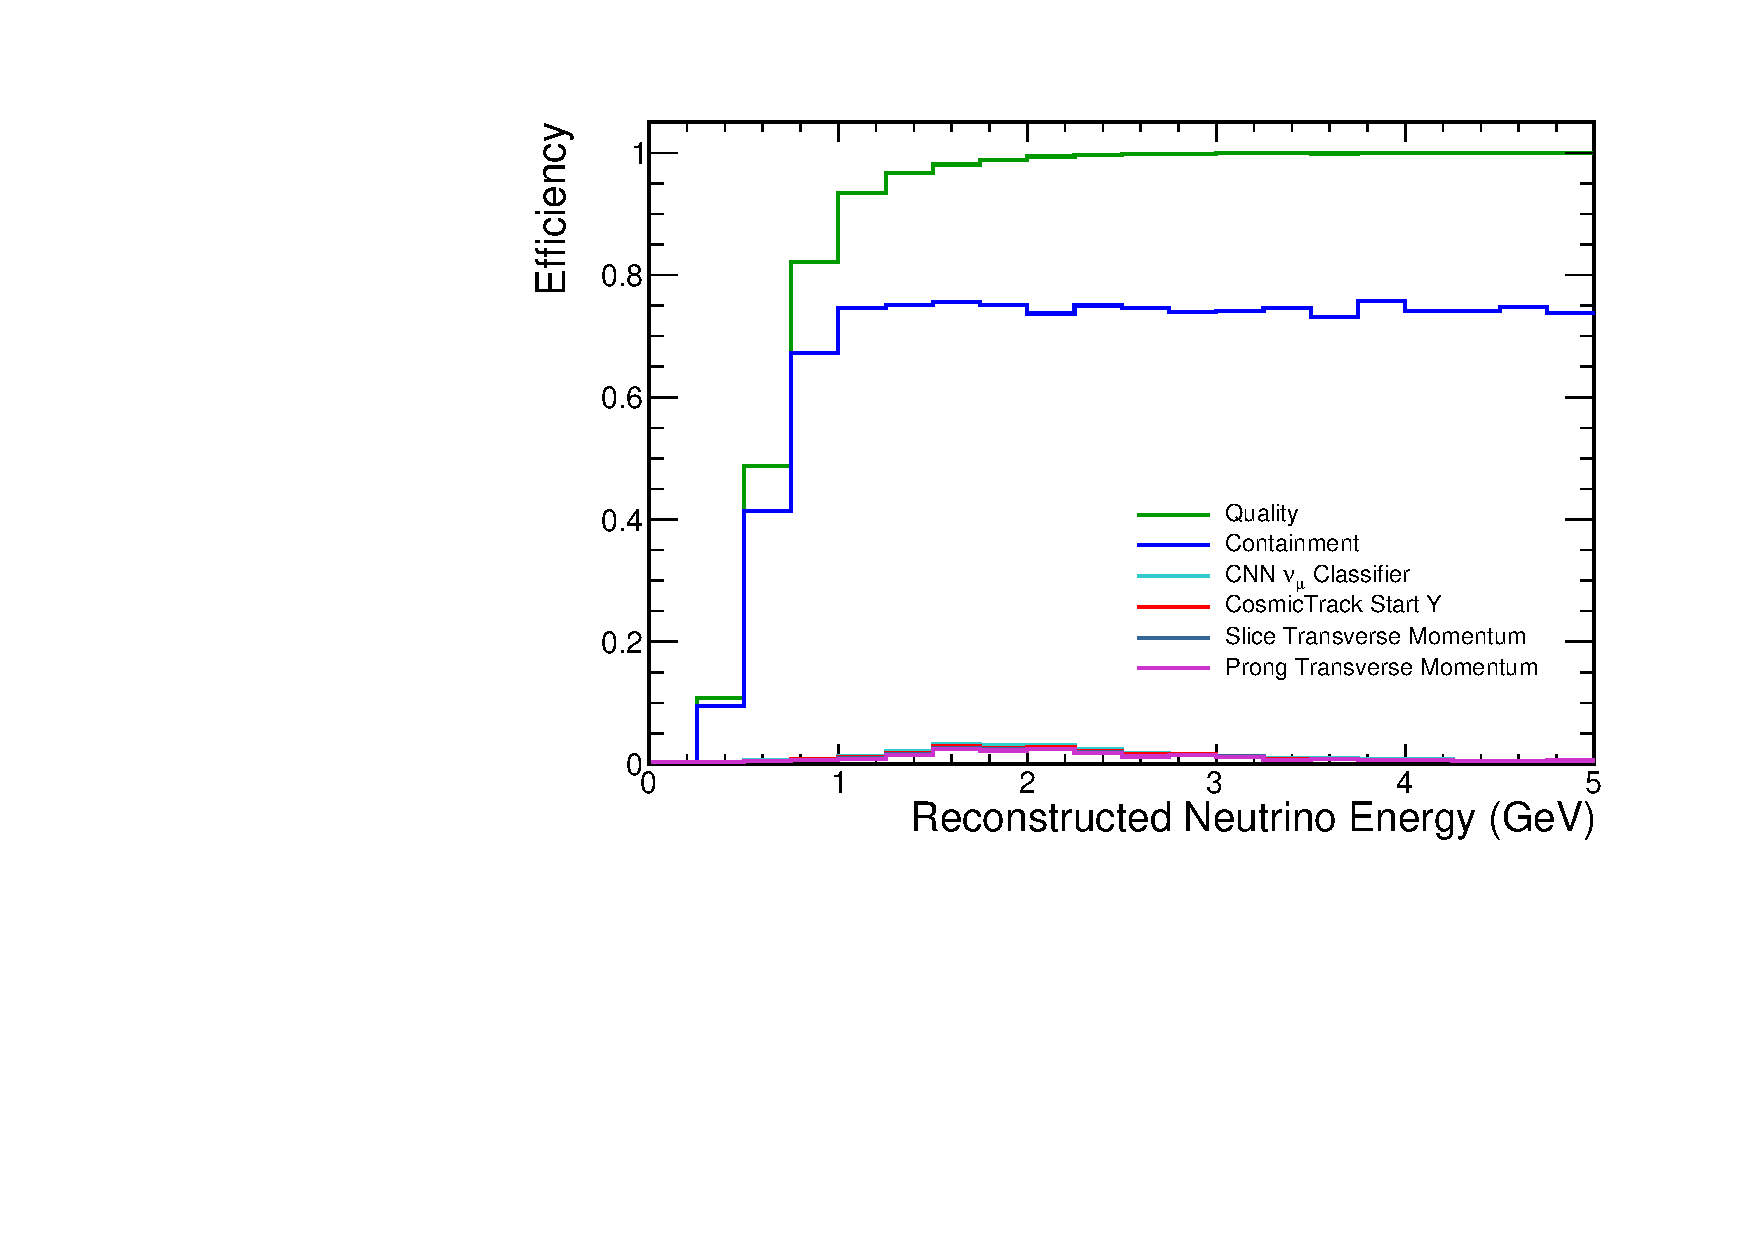
\includegraphics[width=\textwidth]{figures/selection/myflow_bkg_eff_osc.pdf}
  \end{subfigure}

\end{center}
\vspace{-10pt}
\caption{Selected $\nu$ background event spectrum and efficiency}{
The top pane shows the reconstructed neutrino energy spectrum
for selected background events from FD MC simulation.
Truth containment is the sample of events which deposit
no energy outside of the detector, this serves as the denominator
for the efficiency ratio shown in the bottom pane.
Each subsequent spectrum adds an additional selection cut to the sample.
}
\label{cut_flow_bkg}
\end{figure}

\begin{figure}
\vspace{-30pt}
\begin{center}
  \begin{subfigure}[b]{0.7\textwidth}
    \centering
    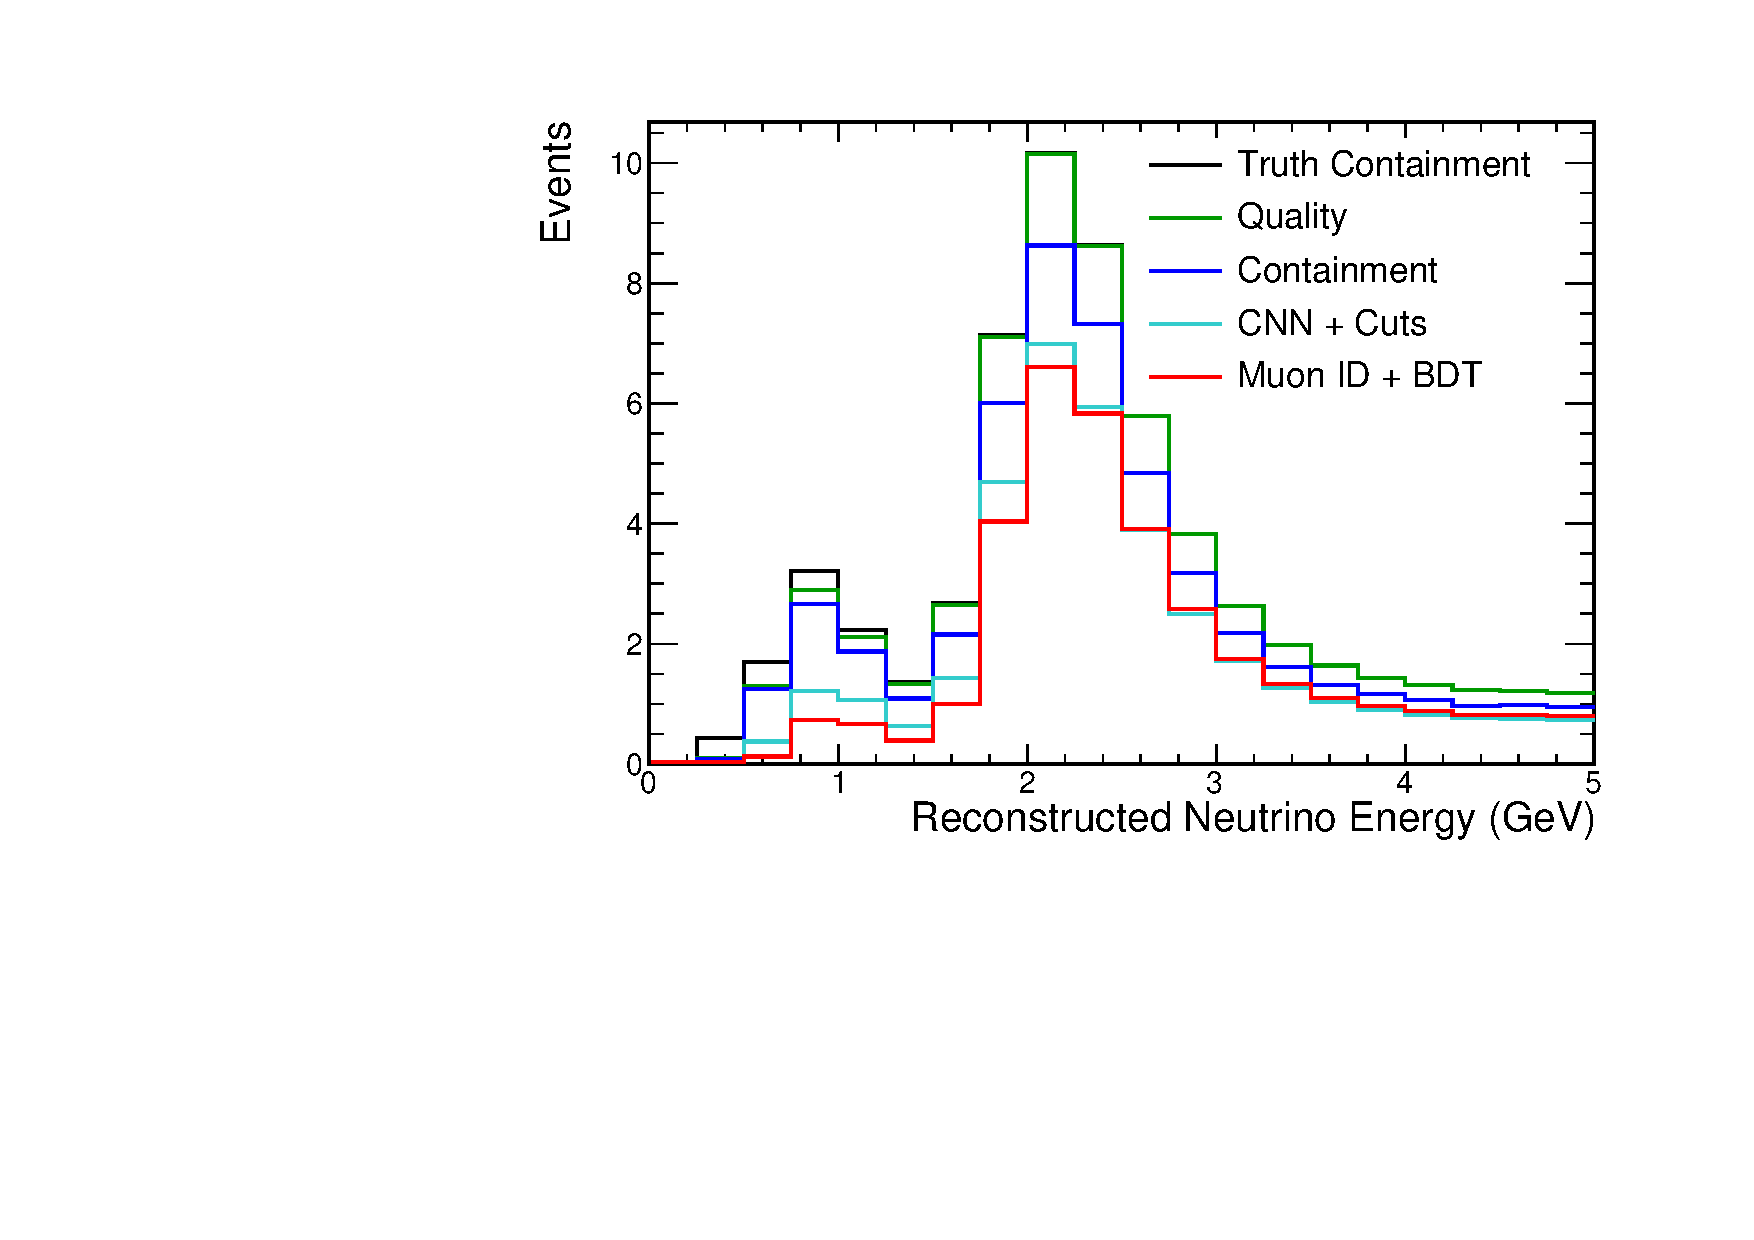
\includegraphics[width=\textwidth]{figures/selection/cosmic_sig_osc.pdf}
  \end{subfigure}

  \begin{subfigure}[b]{0.7\textwidth}
    \centering
    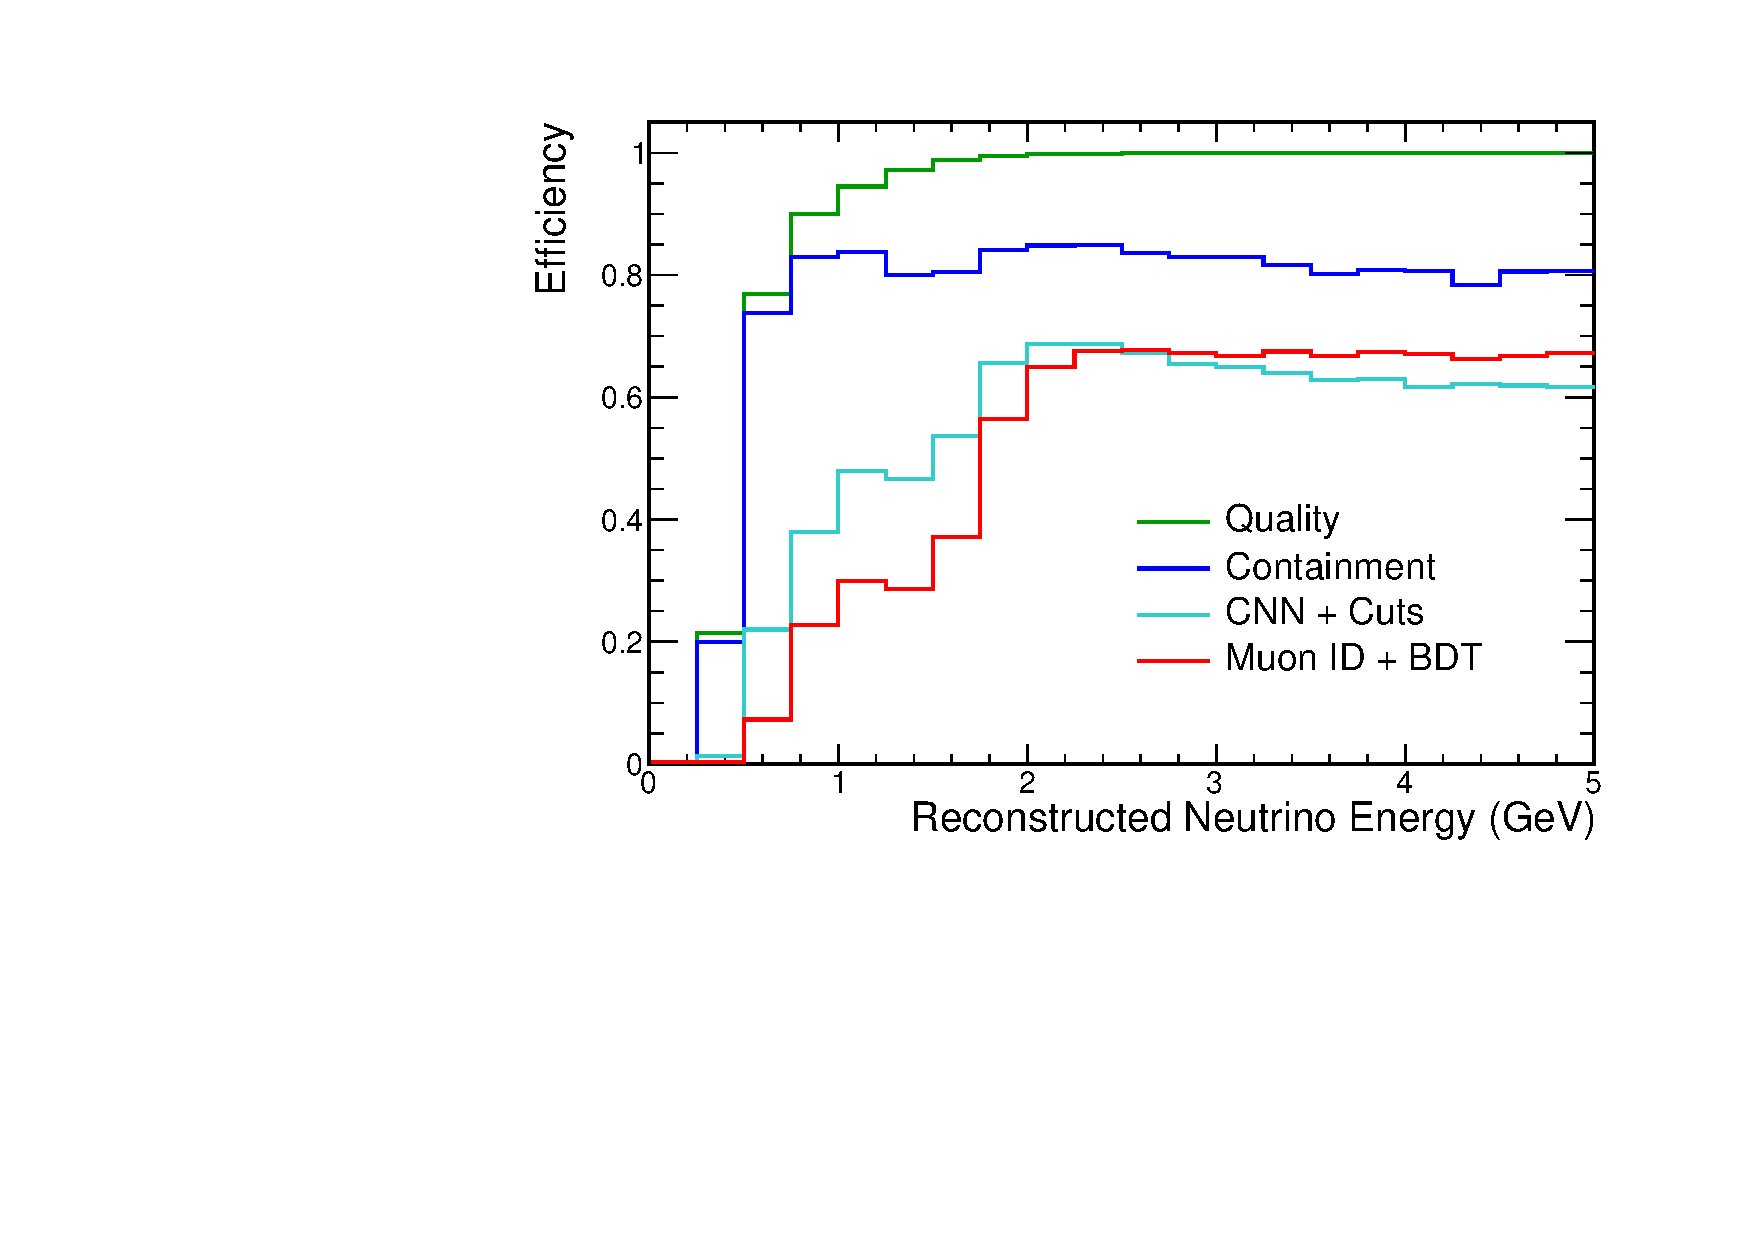
\includegraphics[width=\textwidth]{figures/selection/cosmic_sig_eff_osc.pdf}
  \end{subfigure}

\end{center}
\vspace{-10pt}
\caption{Comparison of \numu CC signal event spectrum and efficiency to
existing approach}{
The top pane shows the reconstructed neutrino energy spectrum
for selected \numu CC signal events from FD MC simulation.
Truth containment is the sample of events which deposit
no energy outside of the detector, this serves as the denominator
for the efficiency ratio shown in the bottom pane.
Each subsequent spectrum adds an additional selection cut to the sample.
The \numu CC signal distribution has had oscillation probabilities applied
based on the true energy of selected events and oscillation parameters
from described in \ref{osc_weight_section}.

The two most selective spectra, \textit{CNN + Cuts} and
\textit{Muon ID + BDT}, compare
the CNN approach to the existing approach used in \cite{nova2016numu}.
The existing approach relied on the Muon ID described in
Section \ref{remid_section}, along with a boosted decision tree
\cite{friedman2002stochastic} to reject cosmic background.
The CNN selection presented here improves the selection efficiency compared to
compared to the existing approach in the low energy bins which are most
sensitive to neutrino oscillation.

}
\label{cut_flow_comp_sig}
\end{figure}

\begin{figure}
\vspace{-30pt}
\begin{center}
  \begin{subfigure}[b]{0.7\textwidth}

    \centering
    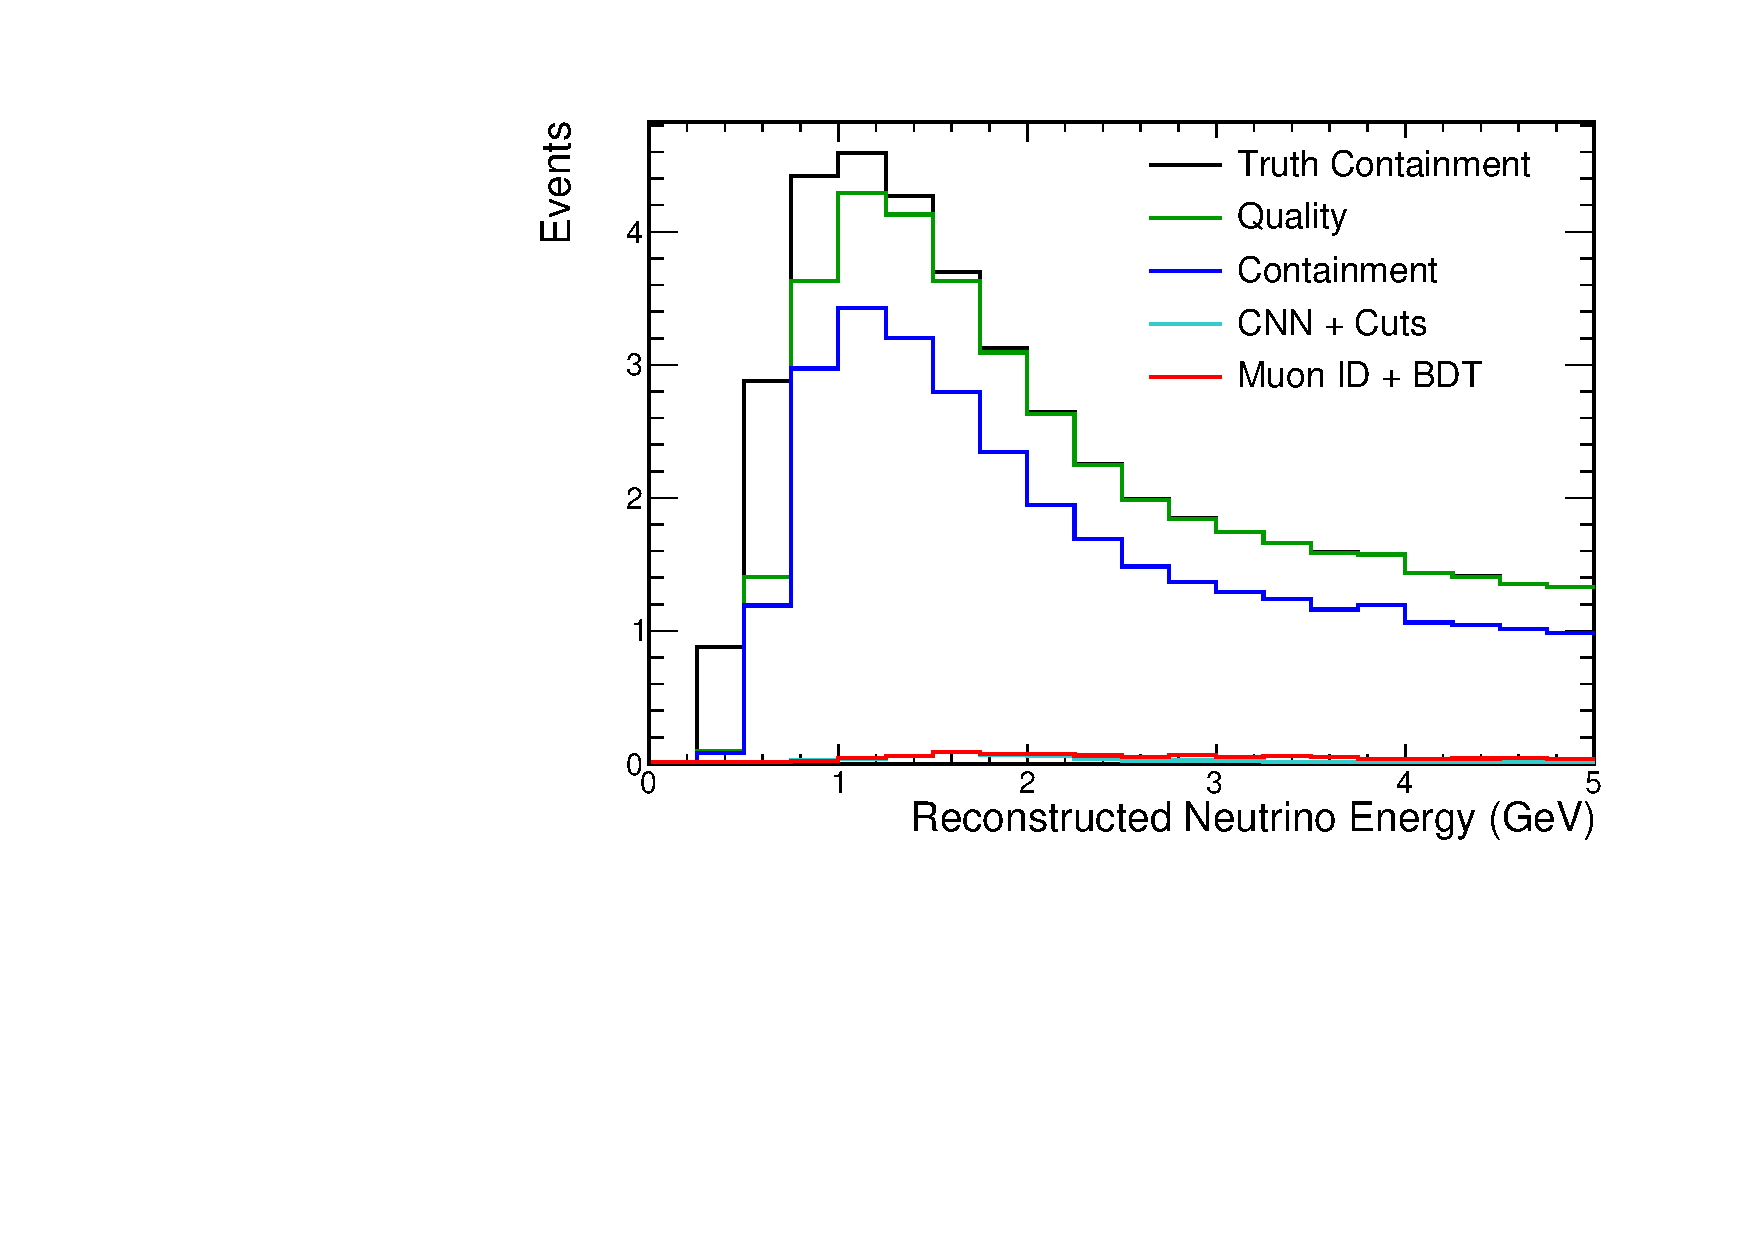
\includegraphics[width=\textwidth]{figures/selection/cosmic_bkg_osc.pdf}
  \end{subfigure}

  \begin{subfigure}[b]{0.7\textwidth}
    \centering
    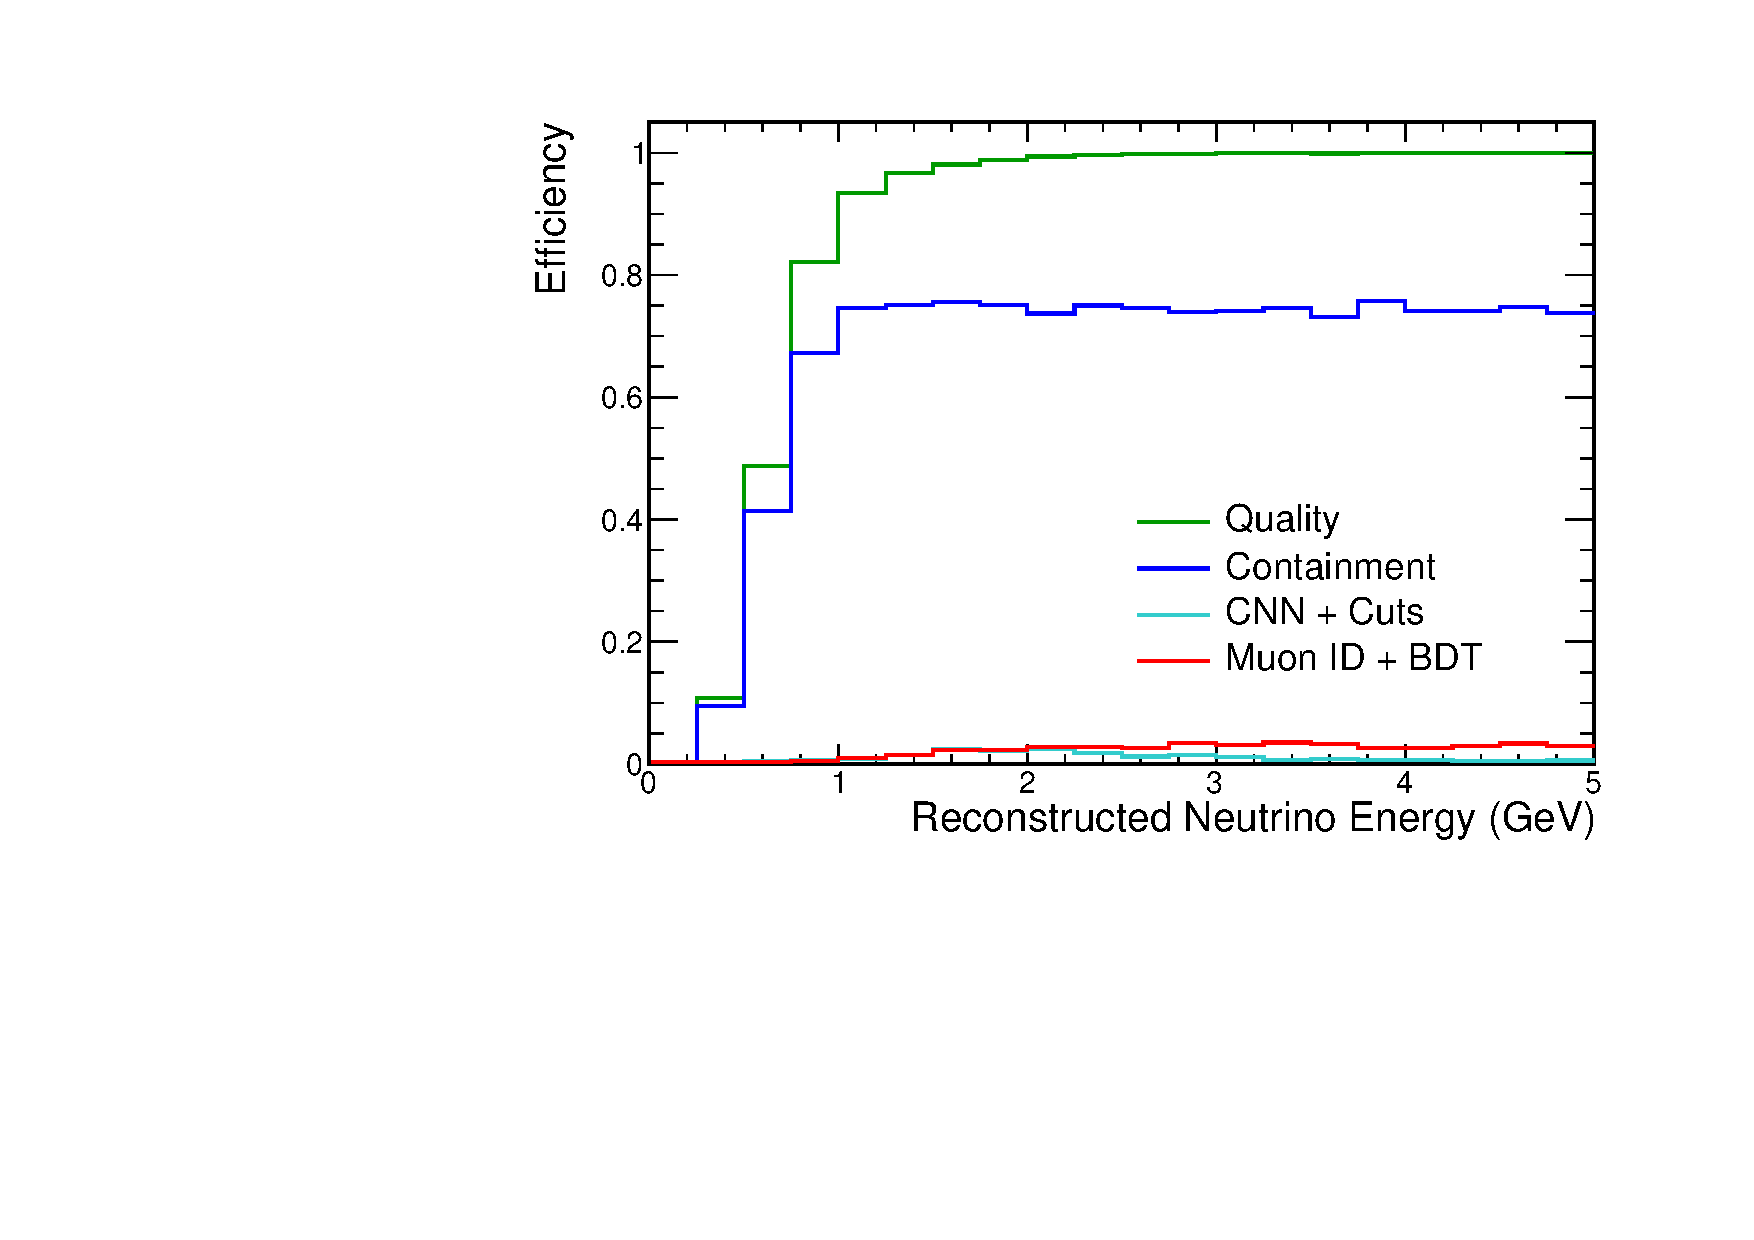
\includegraphics[width=\textwidth]{figures/selection/cosmic_bkg_eff_osc.pdf}
  \end{subfigure}

\end{center}
\vspace{-10pt}
\caption{Comparison of $\nu$ background event spectrum and efficiency to
existing approach}{
The top pane shows the reconstructed neutrino energy spectrum
for selected background events from FD MC simulation.
Truth containment is the sample of events which deposit
no energy outside of the detector, this serves as the denominator
for the efficiency ratio shown in the bottom pane.
Each subsequent spectrum adds an additional selection cut to the sample.

The two most selective spectra, \textit{CNN + Cuts} and
\textit{Muon ID + BDT}, compare
the CNN approach to the existing approach used in \cite{nova2016numu}.
The existing approach relied on the Muon ID described in
Section \ref{remid_section}, along with a boosted decision tree
\cite{friedman2002stochastic} to reject cosmic background.
The CNN selection presented here improves the background rejection efficiency
compared to the existing approach.
}
\label{cut_flow_comp_bkg}
\end{figure}



\begin{figure}
\begin{center}
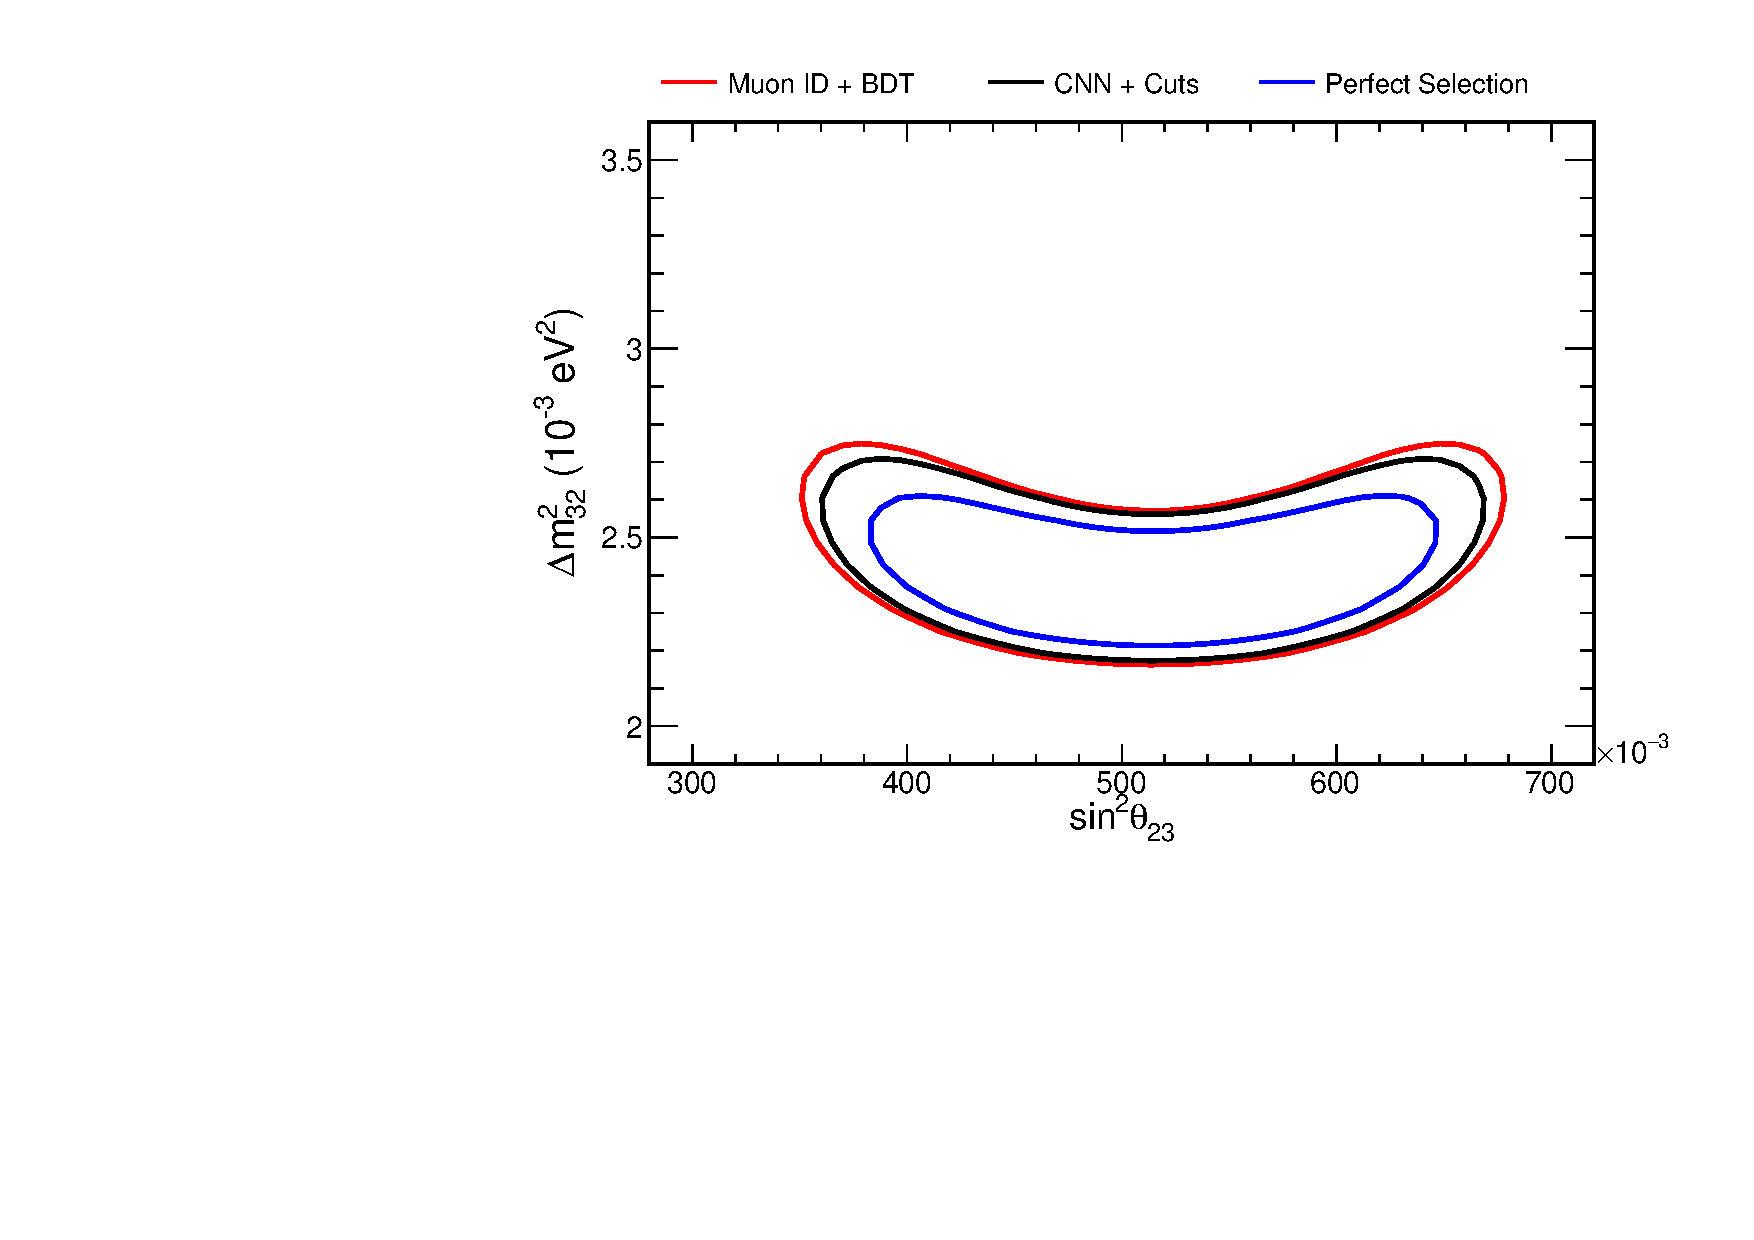
\includegraphics[width=0.9\textwidth]{figures/selection/contoursfhc1cosmic.pdf}
\end{center}
\caption{Sensitivity comparison between existing analysis approach and CNN
technique}{
The contours shown above are expected 90\% confidence limits for \deltamtht
and \thetatth using \nova MC simulation.
Confidence intervals are formed using the procedure described in Section
\ref{fitting_section}, although it should be noted that no extrapolation
is used here; A ``fake data'' scaled oscillated from the FD MC prediction
is fit to the FD MC prediction.
No systematic errors are included.
The red contour uses the selection described in \cite{nova2016numu}, the black
is the CNN approach, and the blue is the result of a perfect selection where
\numu CC events are selected by MC truth.
Contours were generated with oscillation probabilities applied
based on the true energy of selected events and oscillation parameters
from described in \ref{osc_weight_section}.

}
\label{contour_improvement}
\end{figure}
\clearpage

\section{ND Selected Sample}
\label{nd_selection_section}

The ND selection gives an opportunity to compare the MC prediction
to data.
This gives us our first glimpse at detector data induced
by real neutrino interactions.

The agreement between the MC prediction and the data is generally good.
Reconstructed slices (described in section \ref{slicer_section})
show a slight bias in the data toward smaller clusters, as seen in
Figure~\ref{nd_selected_slcNHit}.
The Muon ID data, shown in Figure~\ref{nd_selected_remid}, display
a slight excess in the most signal-like bins relative to the MC prediction.
That excess in signal translates to a normalization enhancement in the
muon track length (Section \ref{kalmantrack_section})
distribution in Figure~\ref{nd_selected_trkLen}.
The singal excess is also visible in the distribution of CNN softmax output
seen in Figure~\ref{nd_selected_cvnmu}.
The shift in Slice \nhit is driven primarily by a discrepancy
in the number of hits in the hadronic cluster (as described in
Section~\ref{energy_section}), which can be seen in Figure~\ref{nd_selected_hadNHit}.
Calorimetric hadronic energy picks up that same shift toward lower energy
relative to the MC prediction.
Since the hadronic energy enters directly into reconstructed neutrino energy,
seen in Figure~\ref{nd_selected_numuE}, a shift is seen there as well.

These discrepancies, especially in the energy spectra,
can be troubling from the perspective of oscillation
analysis.
The extrapolation procedure described in Section~\ref{extrap_section}
will pick up the normalization and shape discrepancies and propagate them
to the FD prediction, but that will be incorrect if the discrepancies
are not correlated to the FD observation.
Thus, we must include systematic errors which account for the discrepancies
between the ND MC prediction and ND data.
The discussion of systematic errors will come in Chapter~\ref{systs_chapter}.

\begin{figure}
\begin{center}
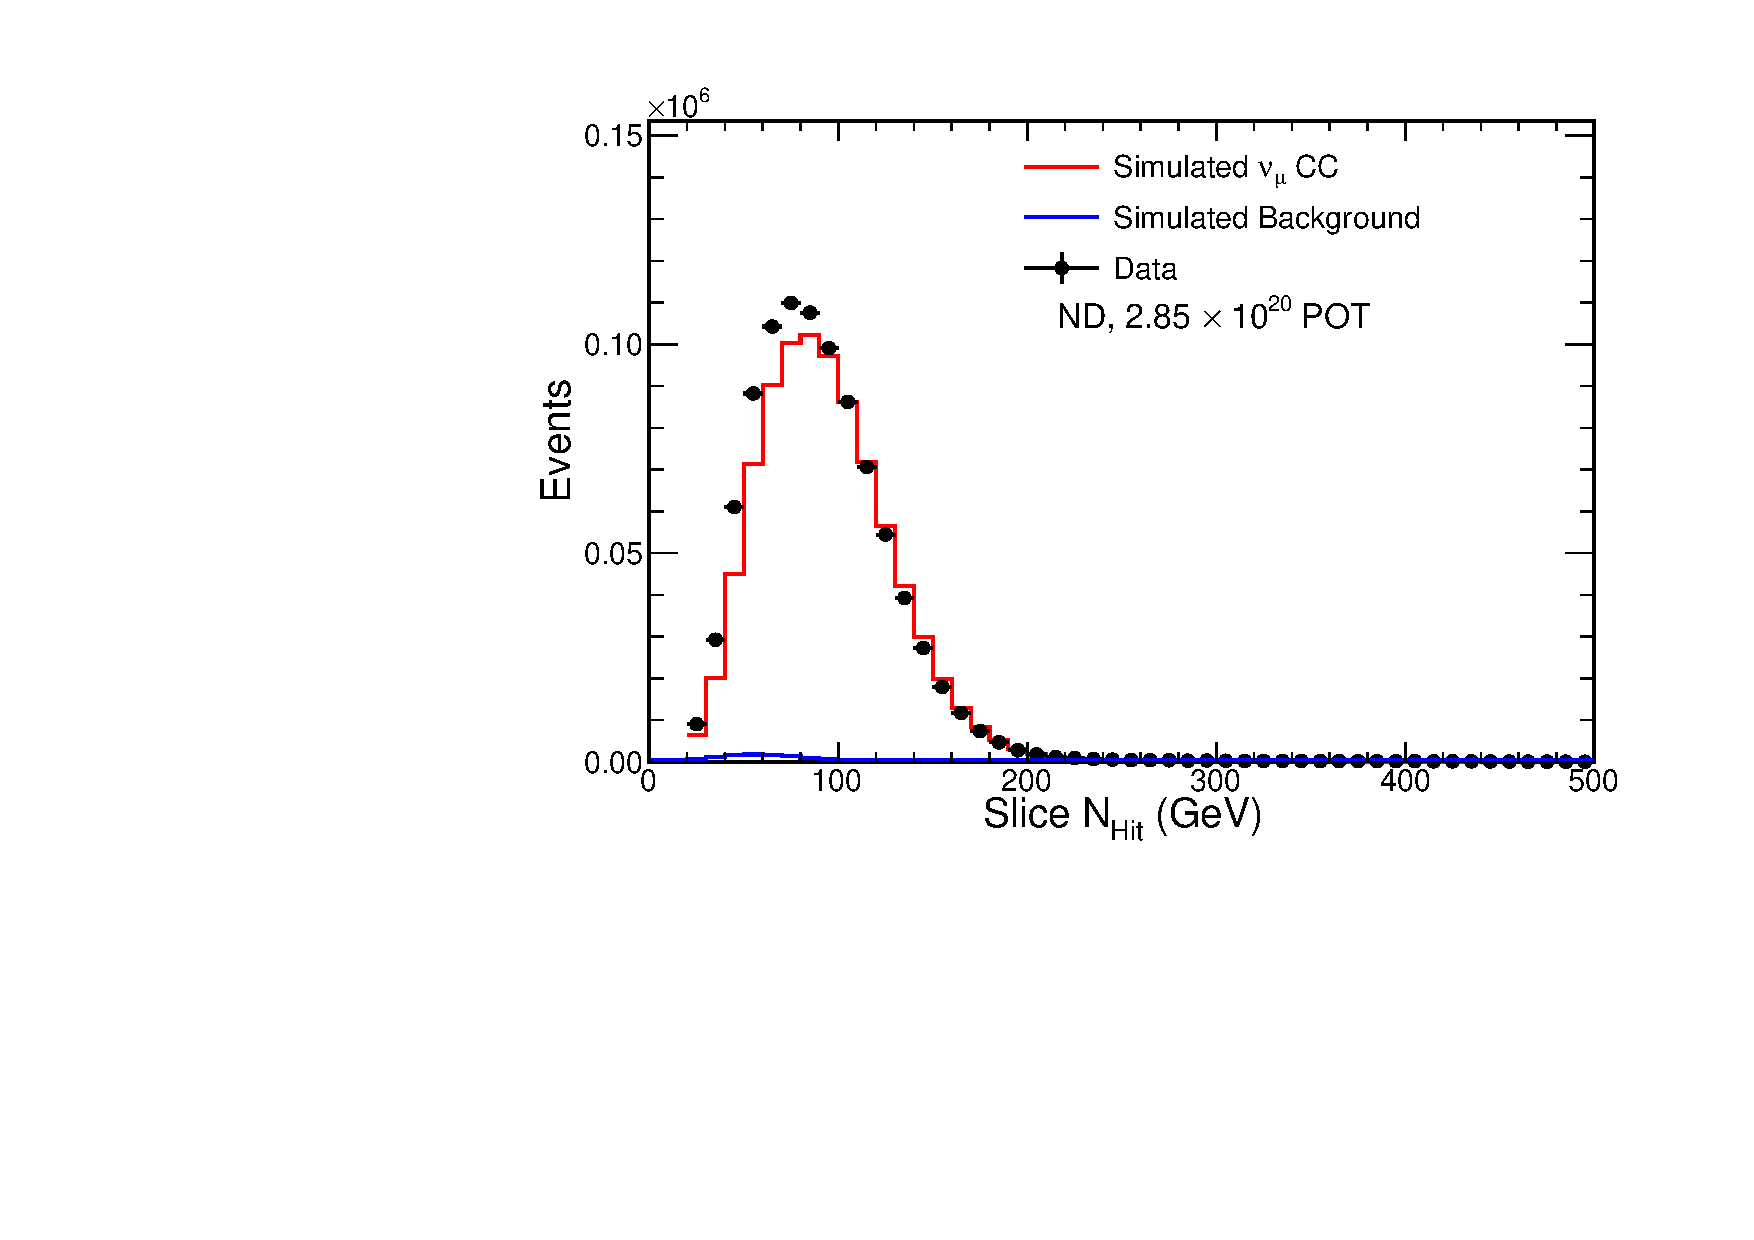
\includegraphics[width=0.9\textwidth]{figures/selection_nd/slcNHit_NumuContainND_CVN.pdf}
\end{center}
\caption{Slice $N_{Hit}$ distribution for selected ND sample}{
Comparing ND data to the ND MC prediction provides a window on simulation
performance.  The MC prediction is shown in red, with the background
component shown in blue.
The selected ND data are shown as black points.
Slice $N_{Hit}$ is the number of hits in the reconstructed slice,
as described in Section \ref{slicer_section}.
The data show a slight shift toward smaller clusters.
}
\label{nd_selected_slcNHit}
\end{figure}


\begin{figure}
\begin{center}
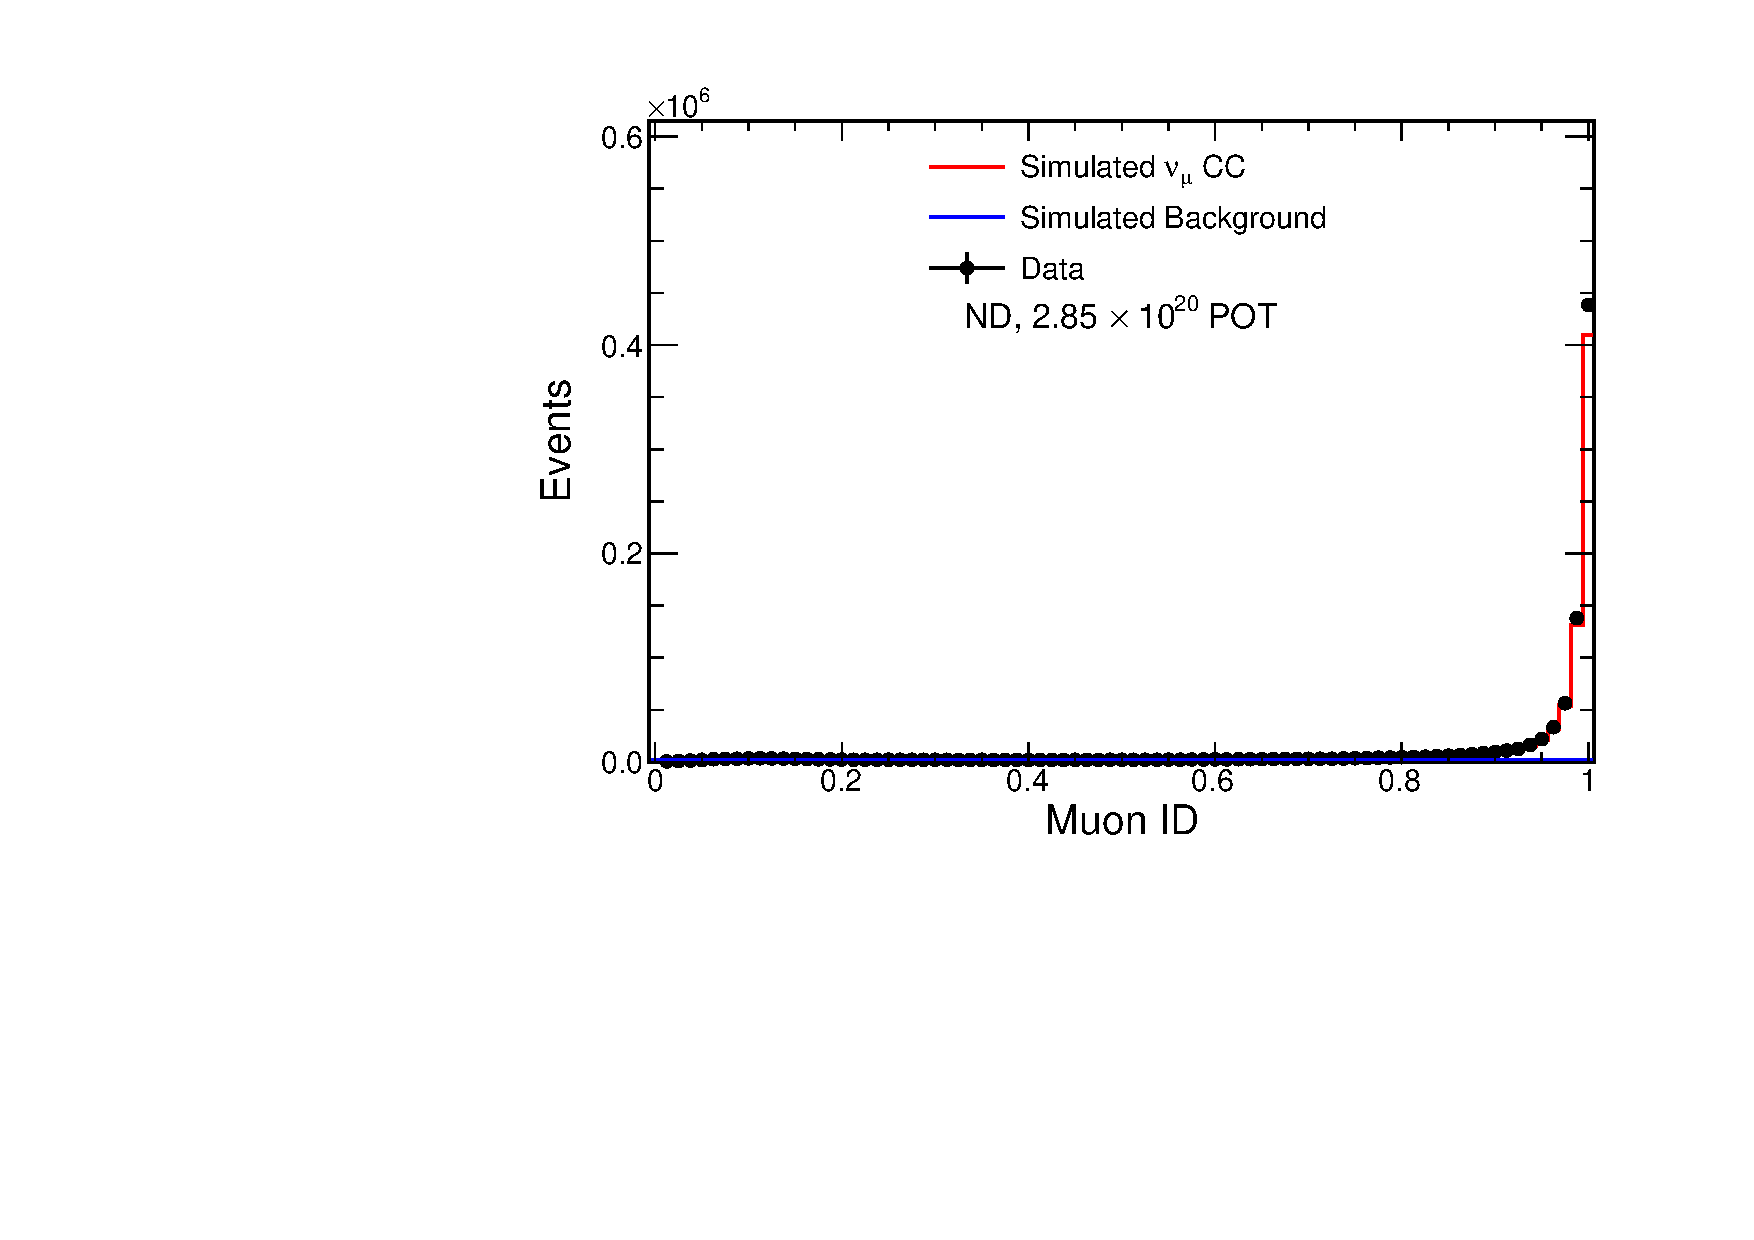
\includegraphics[width=0.9\textwidth]{figures/selection_nd/remid_NumuContainND_CVN.pdf}
\end{center}
\caption{Muon ID distribution for selected ND sample}{
Comparing ND data to the ND MC prediction provides a window on simulation
performance.  The MC prediction is shown in red, with the background
component shown in blue.
The selected ND data are shown as black points.
The Muon ID variable is the output of a kNN based on track length and
likelihood estimates for observed energy deposition and multiple scattering,
as described in Section \ref{remid_section}.}
\label{nd_selected_remid}
\end{figure}

\begin{figure}
\begin{center}
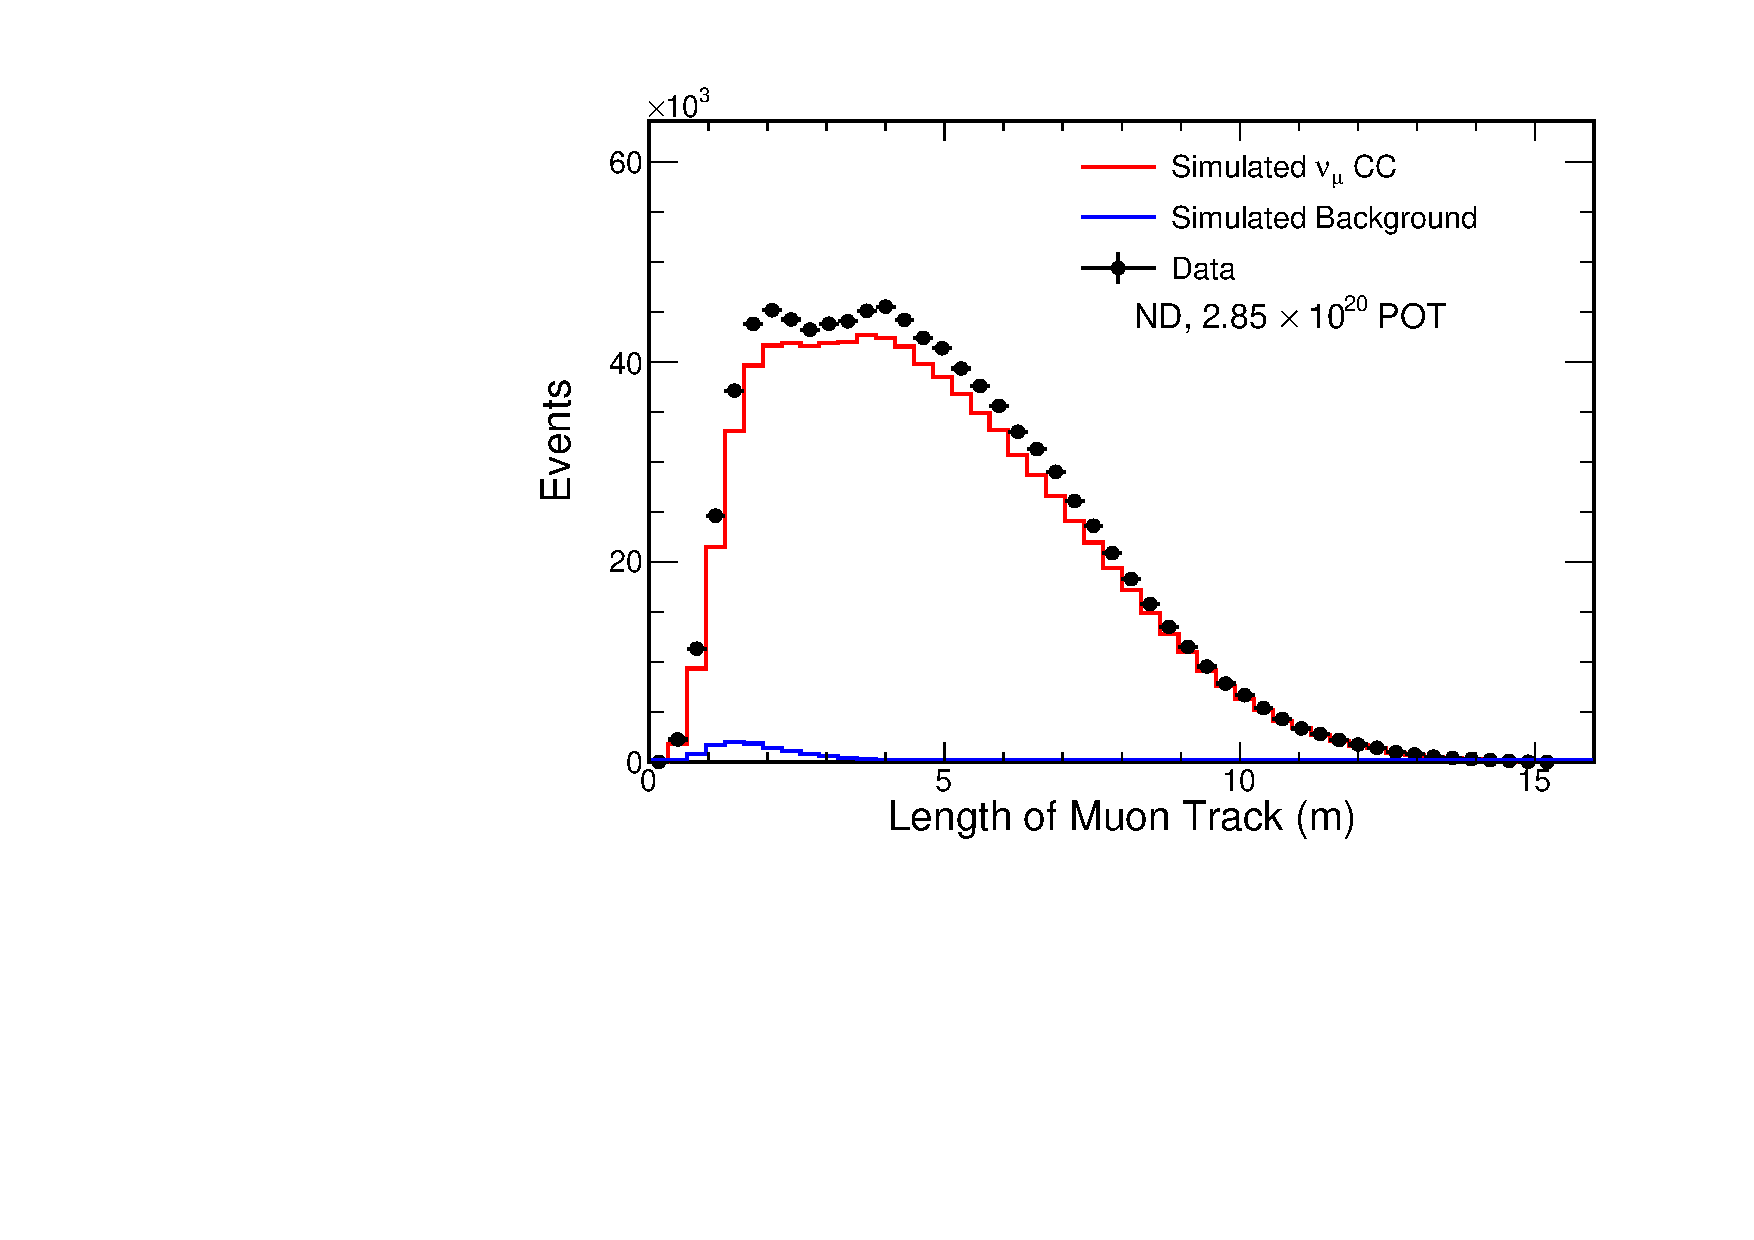
\includegraphics[width=0.9\textwidth]{figures/selection_nd/trkLength_NumuContainND_CVN.pdf}
\end{center}
\caption{Muon track length distribution for selected ND sample}{
Comparing ND data to the ND MC prediction provides a window on simulation
performance.  The MC prediction is shown in red, with the background
component shown in blue.
The selected ND data are shown as black points.
The muon track length is the length of the muon track (Section
\ref{kalmantrack_section})
with the highest muon ID score (Section \ref{remid_section}).
}
\label{nd_selected_trkLen}
\end{figure}

\begin{figure}
\begin{center}
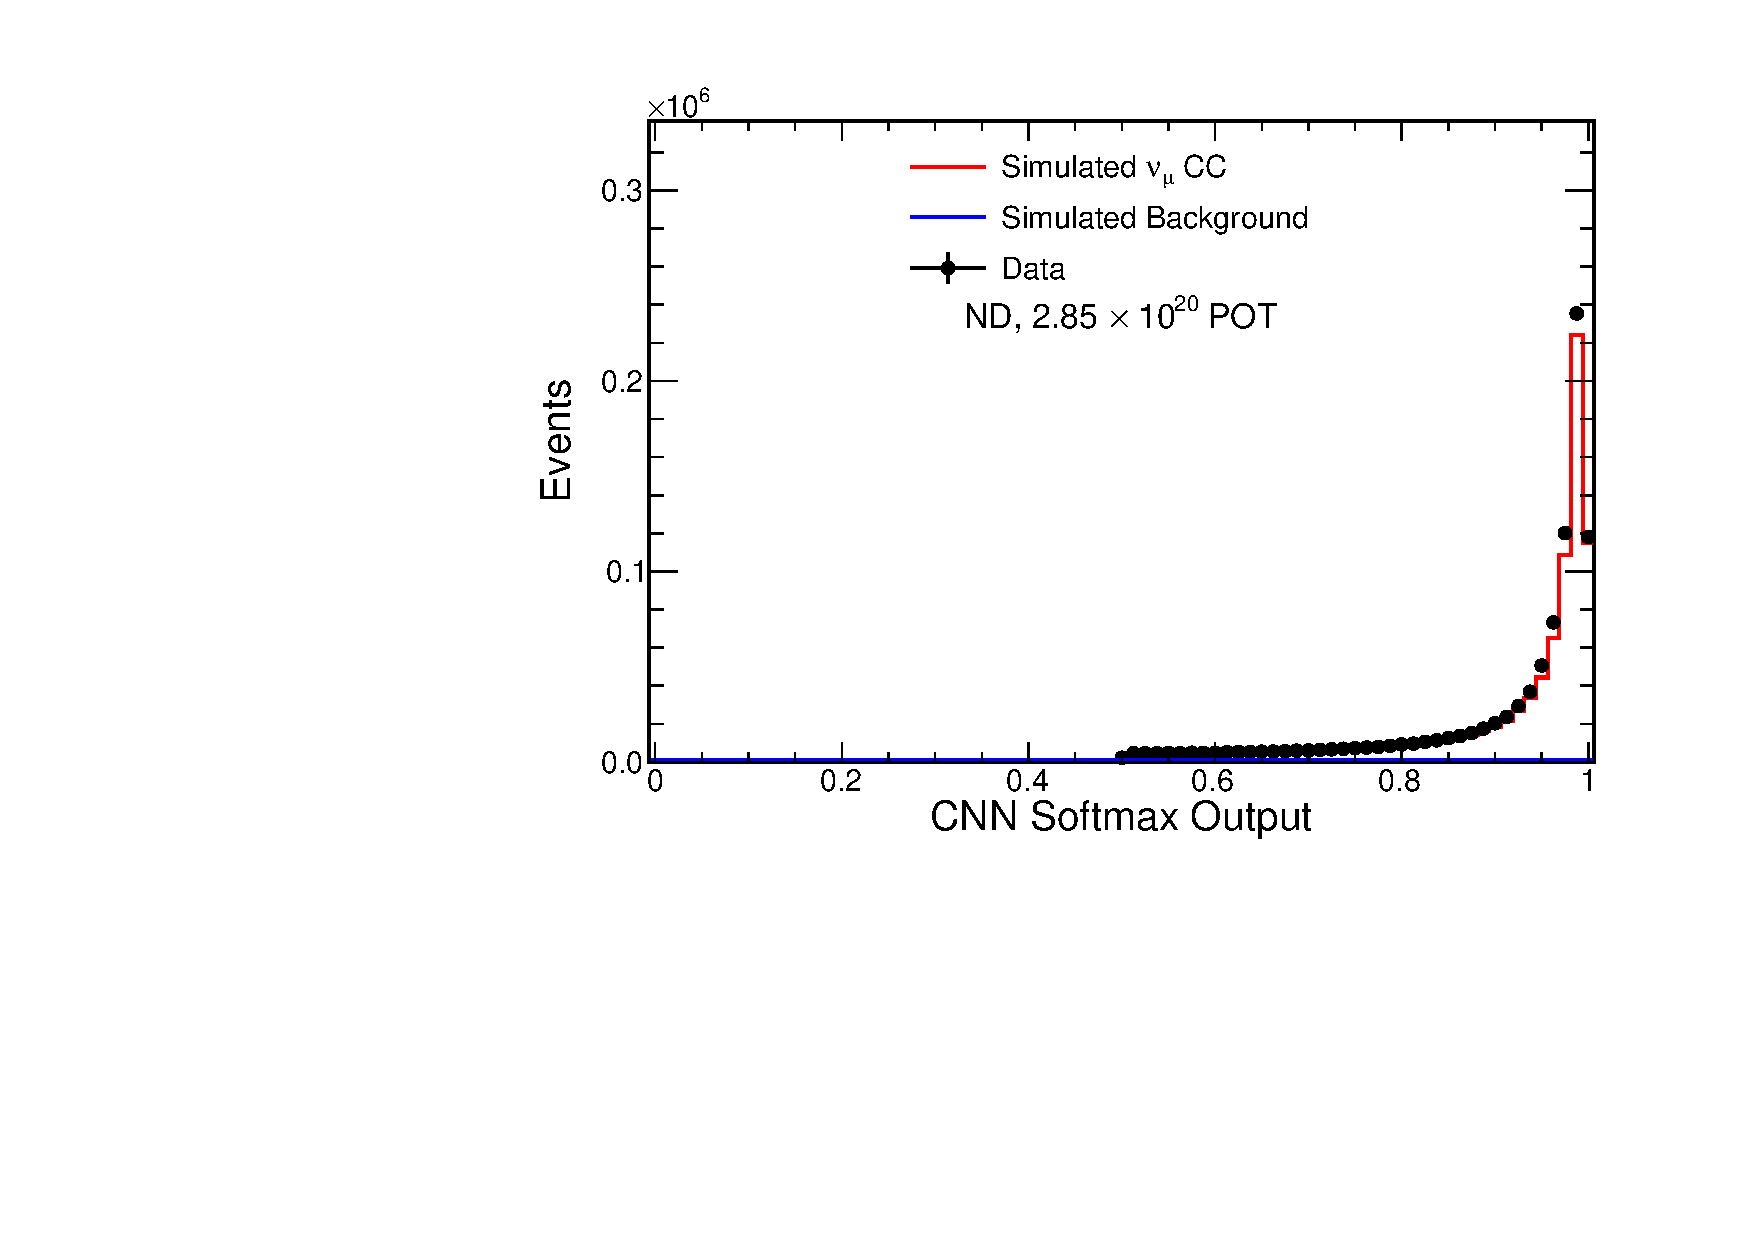
\includegraphics[width=0.9\textwidth]{figures/selection_nd/cvnmu_NumuContainND_CVN.pdf}
\end{center}
\caption{CNN classifier output distribution for selected ND sample}{
Comparing ND data to the ND MC prediction provides a window on simulation
performance.  The MC prediction is shown in red, with the background
component shown in blue.
The selected ND data are shown as black points.
The CNN classifier shows a slight enhancement in the signal region, similar
to the Muon ID varaible shown in Figure \ref{nd_selected_remid}.}
\label{nd_selected_cvnmu}
\end{figure}


\begin{figure}
\begin{center}
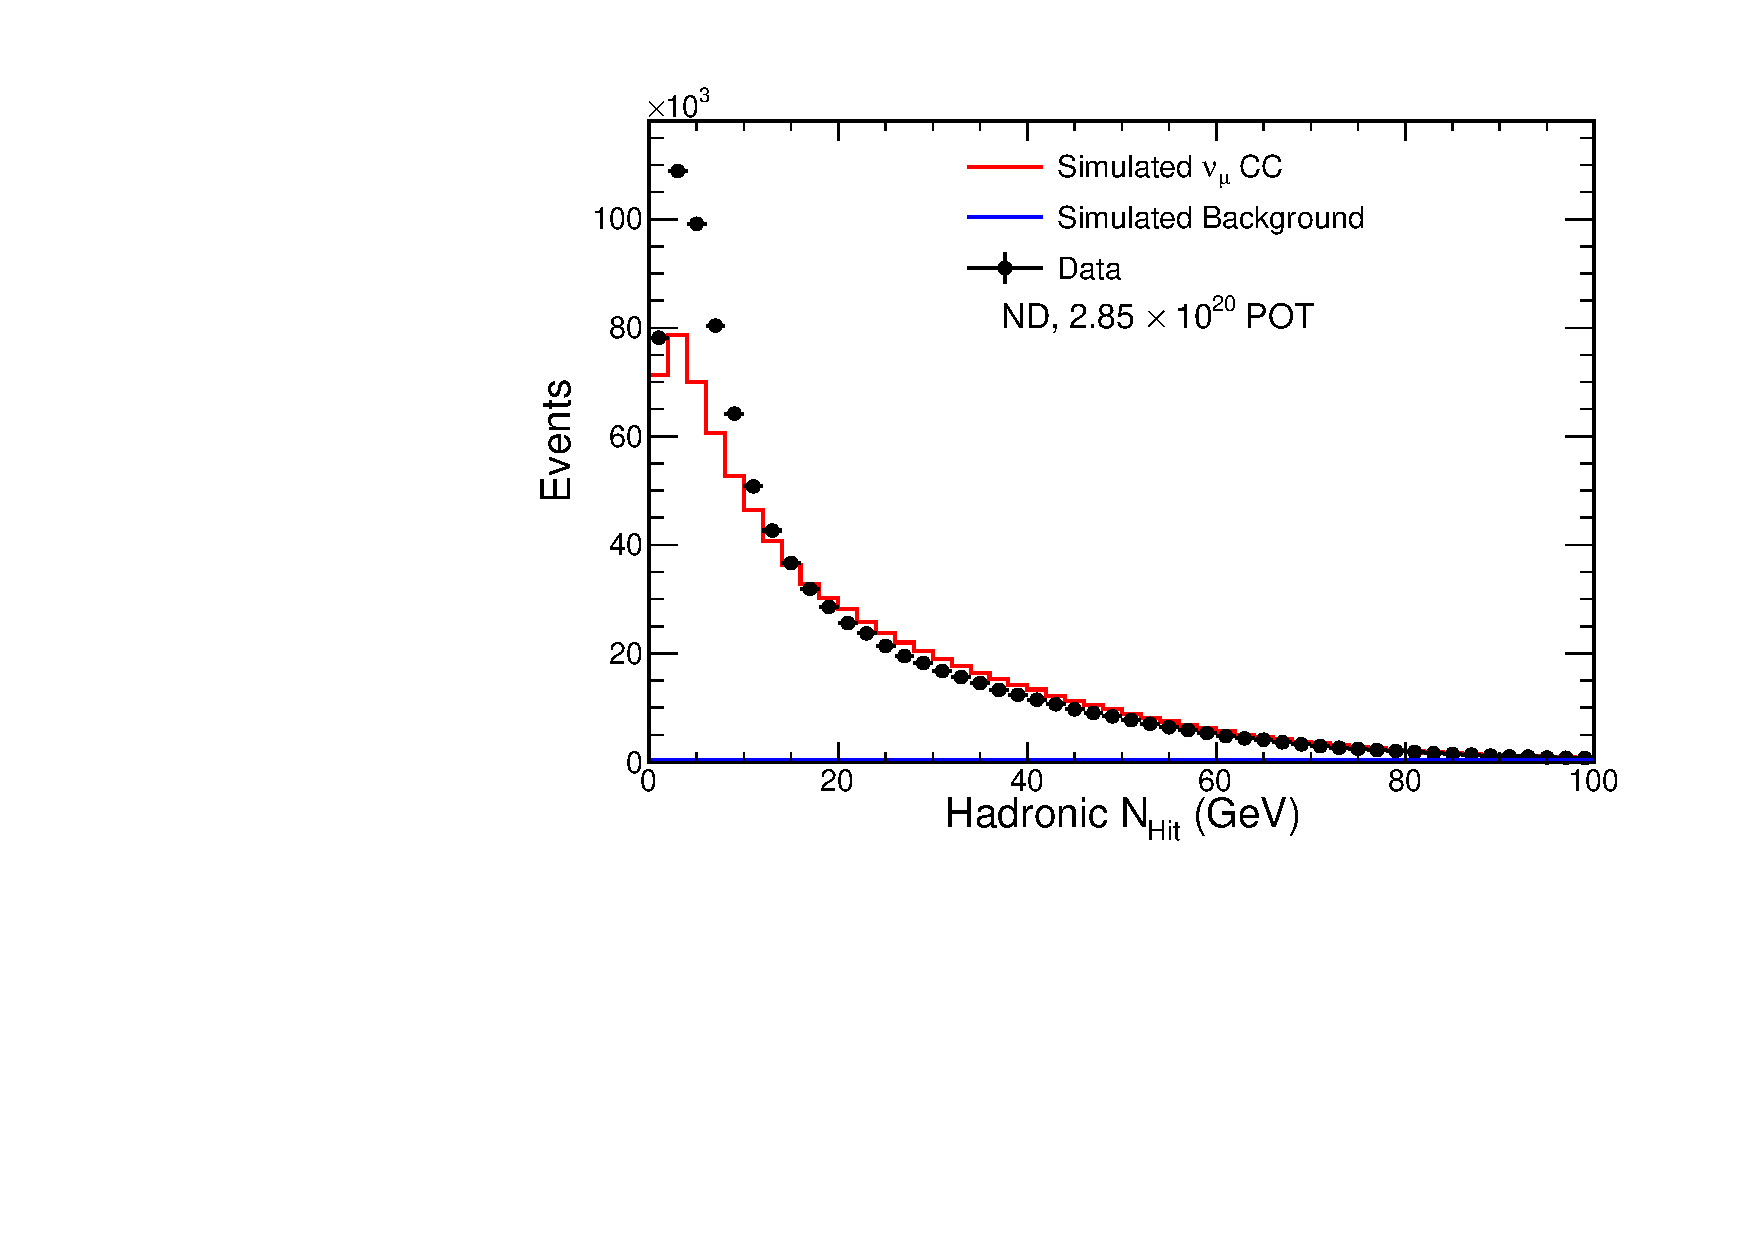
\includegraphics[width=0.9\textwidth]{figures/selection_nd/hadNHit_NumuContainND_CVN.pdf}
\end{center}
\caption{Hadronic cluster $N_{Hit}$ distribution for selected ND sample}{
Comparing ND data to the ND MC prediction provides a window on simulation
performance.  The MC prediction is shown in red, with the background
component shown in blue.
The selected ND data are shown as black points.
This distribution shows the number of hits in the hadronic cluster, that is,
all hits in the slice which are not on the selected muon track,
as described in Section \ref{energy_section}.
The data show a trend toward fewer hits in the hadronic cluster, which is
consistent with \cite{nova2016numu}.}
\label{nd_selected_hadNHit}
\end{figure}

\begin{figure}
\begin{center}
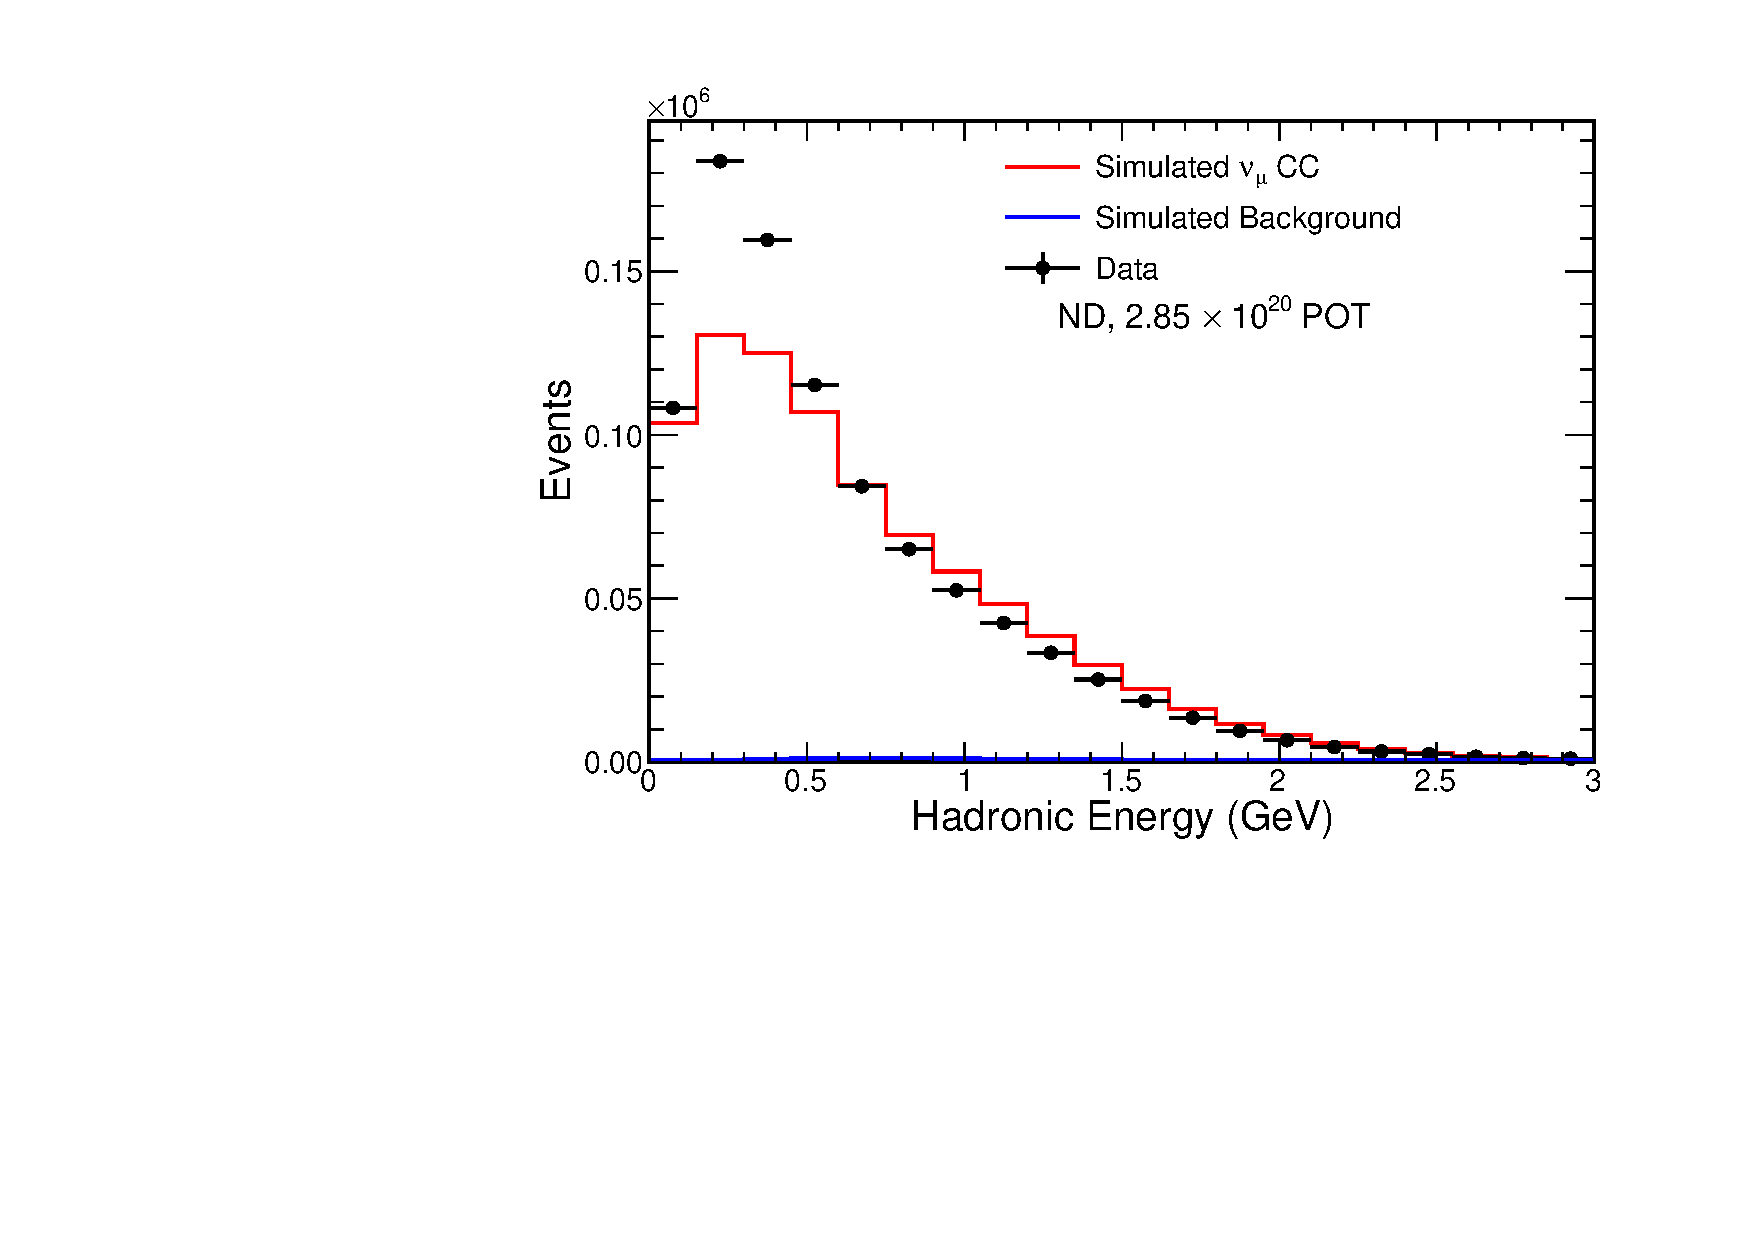
\includegraphics[width=0.9\textwidth]{figures/selection_nd/hadE_NumuContainND_CVN.pdf}
\end{center}
\caption{Hadronic energy distribution for selected ND sample}{
Comparing ND data to the ND MC prediction provides a window on simulation
performance.  The MC prediction is shown in red, with the background
component shown in blue.
The selected ND data are shown as black points.
Hadronic energy is the result of the spline fit to the calorimetric energy
of the hadronic cluster as described in Section \ref{energy_section}.
The data show a shift toward lower hadronic energy, similar to that observed in
from \cite{nova2016numu}.}
\label{nd_selected_hadE}
\end{figure}


\begin{figure}
\begin{center}
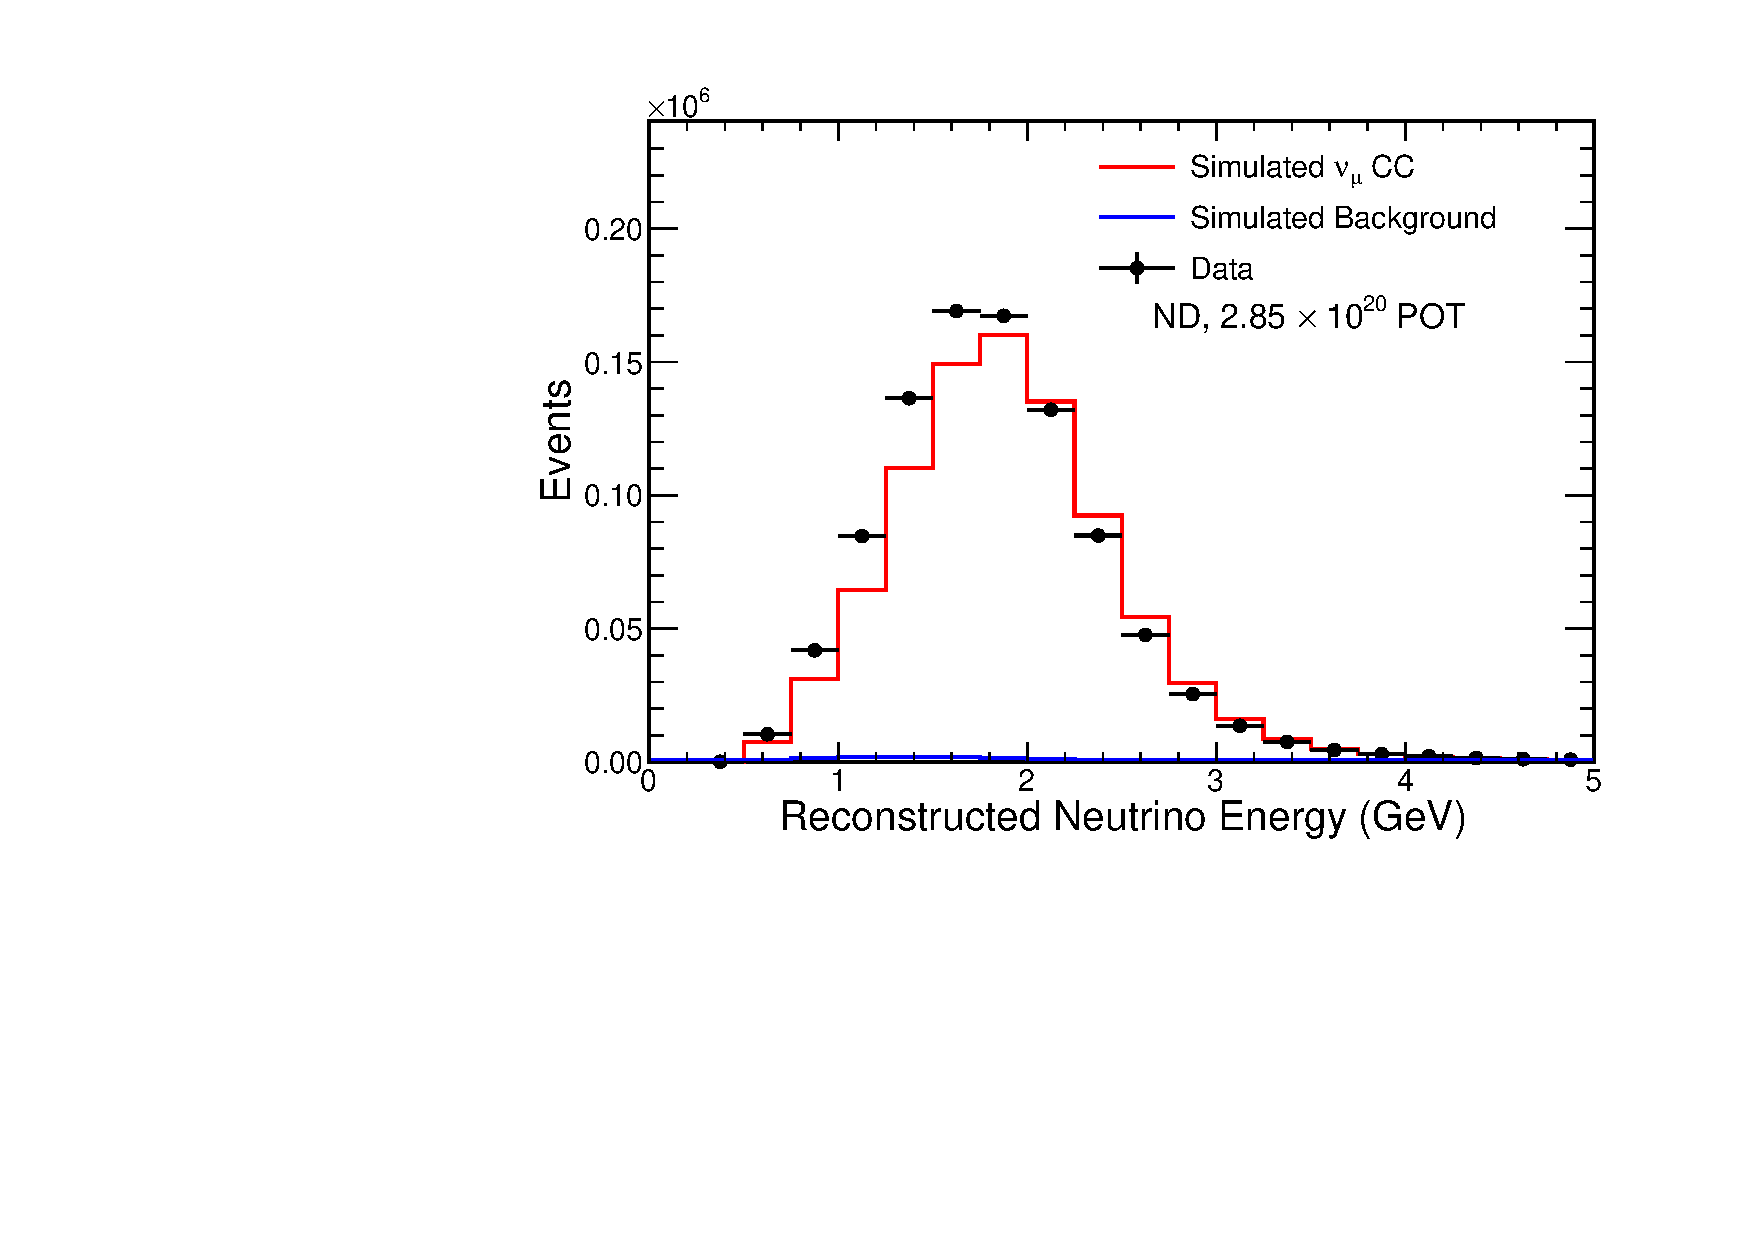
\includegraphics[width=0.9\textwidth]{figures/selection_nd/numuE_NumuContainND_CVN.pdf}
\end{center}
\caption{Reconstructed energy distribution for selected ND sample}{
Comparing ND data to the ND MC prediction provides a window on simulation
performance.  The MC prediction is shown in red, with the background
component shown in blue.
The selected ND data are shown as black points.
Reconstructed energy is the sum of muon track energy and hadronic energy,
as described in section \ref{energy_section}.
The data show a shift toward lower energy, consistent with the
observation in \cite{nova2016numu}.
}
\label{nd_selected_numuE}
\end{figure}


%%%%%%%%%%%%%%%%%%%%%%%%%%%%%%%%%%%%%%%%%%%%%%%%%%%%%%%%%%%%%%%%%%%%%%%%%%%%%%%%
